\documentclass{report}



%%%%%%%%%%%%%%%%%%%%%%%%%%%%%%%%%
% PACKAGE IMPORTS
%%%%%%%%%%%%%%%%%%%%%%%%%%%%%%%%%


% Codificación y tipografía básica (se cargan aquí para orden correcto)
\usepackage[utf8]{inputenc}
\usepackage[T1]{fontenc}
\usepackage{lmodern}
% Idioma español para nombres de elementos flotantes (Figura, Tabla, etc.)
\usepackage[spanish]{babel}
% Asegurar nombre de tablas en español
\addto\captionsspanish{\renewcommand{\tablename}{Tabla}}


\usepackage[tmargin=2cm,rmargin=1in,lmargin=1in,margin=0.85in,bmargin=2cm,footskip=.2in]{geometry}
\usepackage{amsmath,amsfonts,amsthm,amssymb,mathtools}
\usepackage[varbb]{newpxmath}
\usepackage{xfrac}
\usepackage[makeroom]{cancel}
\usepackage{mathtools}
\usepackage{bookmark}
\usepackage{enumitem}
\usepackage{hyperref,theoremref}
\hypersetup{
	pdftitle={Assignment},
	colorlinks=true, linkcolor=gray,citecolor=blue,
	bookmarksnumbered=true,
	bookmarksopen=true
}
\usepackage[most,many,breakable]{tcolorbox}
\usepackage{xcolor}
\usepackage{varwidth}
\usepackage{varwidth}
\usepackage{etoolbox}
%\usepackage{authblk}
\usepackage{nameref}
\usepackage{multicol,array}
\usepackage{tikz-cd}
\usepackage[ruled,vlined,linesnumbered]{algorithm2e}
\usepackage{comment} % enables the use of multi-line comments (\ifx \fi) 
\usepackage{import}
\usepackage{xifthen}
\usepackage{pdfpages}
\usepackage{transparent}

\newcommand\mycommfont[1]{\footnotesize\ttfamily\textcolor{blue}{#1}}
\SetCommentSty{mycommfont}
\newcommand{\incfig}[1]{%
    \def\svgwidth{\columnwidth}
    \import{./figures/}{#1.pdf_tex}
}

\usepackage{tikzsymbols}
\renewcommand\qedsymbol{$\Laughey$}


%\usepackage{import}
%\usepackage{xifthen}
%\usepackage{pdfpages}
%\usepackage{transparent}


%%%%%%%%%%%%%%%%%%%%%%%%%%%%%%
% SELF MADE COLORS
%%%%%%%%%%%%%%%%%%%%%%%%%%%%%%



\definecolor{myg}{RGB}{56, 140, 70}
\definecolor{myb}{RGB}{45, 111, 177}
\definecolor{myr}{RGB}{199, 68, 64}
\definecolor{mytheorembg}{HTML}{F2F2F9}
\definecolor{mytheoremfr}{HTML}{00007B}
\definecolor{mylenmabg}{HTML}{FFFAF8}
\definecolor{mylenmafr}{HTML}{983b0f}
\definecolor{mypropbg}{HTML}{f2fbfc}
\definecolor{mypropfr}{HTML}{191971}
\definecolor{myexamplebg}{HTML}{F2FBF8}
\definecolor{myexamplefr}{HTML}{88D6D1}
\definecolor{myexampleti}{HTML}{2A7F7F}
\definecolor{mydefinitbg}{HTML}{E5E5FF}
\definecolor{mydefinitfr}{HTML}{3F3FA3}
\definecolor{notesgreen}{RGB}{0,162,0}
\definecolor{myp}{RGB}{197, 92, 212}
\definecolor{mygr}{HTML}{2C3338}
\definecolor{myred}{RGB}{127,0,0}
\definecolor{myyellow}{RGB}{169,121,69}
\definecolor{myexercisebg}{HTML}{F2FBF8}
\definecolor{myexercisefg}{HTML}{88D6D1}


%%%%%%%%%%%%%%%%%%%%%%%%%%%%
% TCOLORBOX SETUPS
%%%%%%%%%%%%%%%%%%%%%%%%%%%%

\setlength{\parindent}{1cm}
%================================
% THEOREM BOX
%================================

\tcbuselibrary{theorems,skins,hooks}
\newtcbtheorem[number within=section]{Theorem}{Theorem}
{%
	enhanced,
	breakable,
	colback = mytheorembg,
	frame hidden,
	boxrule = 0sp,
	borderline west = {2pt}{0pt}{mytheoremfr},
	sharp corners,
	detach title,
	before upper = \tcbtitle\par\smallskip,
	coltitle = mytheoremfr,
	fonttitle = \bfseries\sffamily,
	description font = \mdseries,
	separator sign none,
	segmentation style={solid, mytheoremfr},
}
{th}

\tcbuselibrary{theorems,skins,hooks}
\newtcbtheorem[number within=chapter]{theorem}{Theorem}
{%
	enhanced,
	breakable,
	colback = mytheorembg,
	frame hidden,
	boxrule = 0sp,
	borderline west = {2pt}{0pt}{mytheoremfr},
	sharp corners,
	detach title,
	before upper = \tcbtitle\par\smallskip,
	coltitle = mytheoremfr,
	fonttitle = \bfseries\sffamily,
	description font = \mdseries,
	separator sign none,
	segmentation style={solid, mytheoremfr},
}
{th}


\tcbuselibrary{theorems,skins,hooks}
\newtcolorbox{Theoremcon}
{%
	enhanced
	,breakable
	,colback = mytheorembg
	,frame hidden
	,boxrule = 0sp
	,borderline west = {2pt}{0pt}{mytheoremfr}
	,sharp corners
	,description font = \mdseries
	,separator sign none
}

%================================
% Corollery
%================================
\tcbuselibrary{theorems,skins,hooks}
\newtcbtheorem[number within=section]{Corollary}{Corollary}
{%
	enhanced
	,breakable
	,colback = myp!10
	,frame hidden
	,boxrule = 0sp
	,borderline west = {2pt}{0pt}{myp!85!black}
	,sharp corners
	,detach title
	,before upper = \tcbtitle\par\smallskip
	,coltitle = myp!85!black
	,fonttitle = \bfseries\sffamily
	,description font = \mdseries
	,separator sign none
	,segmentation style={solid, myp!85!black}
}
{th}
\tcbuselibrary{theorems,skins,hooks}
\newtcbtheorem[number within=chapter]{corollary}{Corollary}
{%
	enhanced
	,breakable
	,colback = myp!10
	,frame hidden
	,boxrule = 0sp
	,borderline west = {2pt}{0pt}{myp!85!black}
	,sharp corners
	,detach title
	,before upper = \tcbtitle\par\smallskip
	,coltitle = myp!85!black
	,fonttitle = \bfseries\sffamily
	,description font = \mdseries
	,separator sign none
	,segmentation style={solid, myp!85!black}
}
{th}


%================================
% LENMA
%================================

\tcbuselibrary{theorems,skins,hooks}
\newtcbtheorem[number within=section]{Lenma}{Lenma}
{%
	enhanced,
	breakable,
	colback = mylenmabg,
	frame hidden,
	boxrule = 0sp,
	borderline west = {2pt}{0pt}{mylenmafr},
	sharp corners,
	detach title,
	before upper = \tcbtitle\par\smallskip,
	coltitle = mylenmafr,
	fonttitle = \bfseries\sffamily,
	description font = \mdseries,
	separator sign none,
	segmentation style={solid, mylenmafr},
}
{th}

\tcbuselibrary{theorems,skins,hooks}
\newtcbtheorem[number within=chapter]{lenma}{Lenma}
{%
	enhanced,
	breakable,
	colback = mylenmabg,
	frame hidden,
	boxrule = 0sp,
	borderline west = {2pt}{0pt}{mylenmafr},
	sharp corners,
	detach title,
	before upper = \tcbtitle\par\smallskip,
	coltitle = mylenmafr,
	fonttitle = \bfseries\sffamily,
	description font = \mdseries,
	separator sign none,
	segmentation style={solid, mylenmafr},
}
{th}


%================================
% PROPOSITION
%================================

\tcbuselibrary{theorems,skins,hooks}
\newtcbtheorem[number within=section]{Prop}{Proposition}
{%
	enhanced,
	breakable,
	colback = mypropbg,
	frame hidden,
	boxrule = 0sp,
	borderline west = {2pt}{0pt}{mypropfr},
	sharp corners,
	detach title,
	before upper = \tcbtitle\par\smallskip,
	coltitle = mypropfr,
	fonttitle = \bfseries\sffamily,
	description font = \mdseries,
	separator sign none,
	segmentation style={solid, mypropfr},
}
{th}

\tcbuselibrary{theorems,skins,hooks}
\newtcbtheorem[number within=chapter]{prop}{Proposition}
{%
	enhanced,
	breakable,
	colback = mypropbg,
	frame hidden,
	boxrule = 0sp,
	borderline west = {2pt}{0pt}{mypropfr},
	sharp corners,
	detach title,
	before upper = \tcbtitle\par\smallskip,
	coltitle = mypropfr,
	fonttitle = \bfseries\sffamily,
	description font = \mdseries,
	separator sign none,
	segmentation style={solid, mypropfr},
}
{th}


%================================
% CLAIM
%================================

\tcbuselibrary{theorems,skins,hooks}
\newtcbtheorem[number within=section]{claim}{Claim}
{%
	enhanced
	,breakable
	,colback = myg!10
	,frame hidden
	,boxrule = 0sp
	,borderline west = {2pt}{0pt}{myg}
	,sharp corners
	,detach title
	,before upper = \tcbtitle\par\smallskip
	,coltitle = myg!85!black
	,fonttitle = \bfseries\sffamily
	,description font = \mdseries
	,separator sign none
	,segmentation style={solid, myg!85!black}
}
{th}



%================================
% Exercise
%================================

\tcbuselibrary{theorems,skins,hooks}
\newtcbtheorem[number within=section]{Exercise}{Exercise}
{%
	enhanced,
	breakable,
	colback = myexercisebg,
	frame hidden,
	boxrule = 0sp,
	borderline west = {2pt}{0pt}{myexercisefg},
	sharp corners,
	detach title,
	before upper = \tcbtitle\par\smallskip,
	coltitle = myexercisefg,
	fonttitle = \bfseries\sffamily,
	description font = \mdseries,
	separator sign none,
	segmentation style={solid, myexercisefg},
}
{th}

\tcbuselibrary{theorems,skins,hooks}
\newtcbtheorem[number within=chapter]{exercise}{Exercise}
{%
	enhanced,
	breakable,
	colback = myexercisebg,
	frame hidden,
	boxrule = 0sp,
	borderline west = {2pt}{0pt}{myexercisefg},
	sharp corners,
	detach title,
	before upper = \tcbtitle\par\smallskip,
	coltitle = myexercisefg,
	fonttitle = \bfseries\sffamily,
	description font = \mdseries,
	separator sign none,
	segmentation style={solid, myexercisefg},
}
{th}

%================================
% EXAMPLE BOX
%================================

\newtcbtheorem[number within=section]{Example}{Example}
{%
	colback = myexamplebg
	,breakable
	,colframe = myexamplefr
	,coltitle = myexampleti
	,boxrule = 1pt
	,sharp corners
	,detach title
	,before upper=\tcbtitle\par\smallskip
	,fonttitle = \bfseries
	,description font = \mdseries
	,separator sign none
	,description delimiters parenthesis
}
{ex}

\newtcbtheorem[number within=chapter]{example}{Example}
{%
	colback = myexamplebg
	,breakable
	,colframe = myexamplefr
	,coltitle = myexampleti
	,boxrule = 1pt
	,sharp corners
	,detach title
	,before upper=\tcbtitle\par\smallskip
	,fonttitle = \bfseries
	,description font = \mdseries
	,separator sign none
	,description delimiters parenthesis
}
{ex}

%================================
% DEFINITION BOX
%================================

\newtcbtheorem[number within=section]{Definition}{Definition}{enhanced,
	before skip=2mm,after skip=2mm, colback=red!5,colframe=red!80!black,boxrule=0.5mm,
	attach boxed title to top left={xshift=1cm,yshift*=1mm-\tcboxedtitleheight}, varwidth boxed title*=-3cm,
	boxed title style={frame code={
					\path[fill=tcbcolback]
					([yshift=-1mm,xshift=-1mm]frame.north west)
					arc[start angle=0,end angle=180,radius=1mm]
					([yshift=-1mm,xshift=1mm]frame.north east)
					arc[start angle=180,end angle=0,radius=1mm];
					\path[left color=tcbcolback!60!black,right color=tcbcolback!60!black,
						middle color=tcbcolback!80!black]
					([xshift=-2mm]frame.north west) -- ([xshift=2mm]frame.north east)
					[rounded corners=1mm]-- ([xshift=1mm,yshift=-1mm]frame.north east)
					-- (frame.south east) -- (frame.south west)
					-- ([xshift=-1mm,yshift=-1mm]frame.north west)
					[sharp corners]-- cycle;
				},interior engine=empty,
		},
	fonttitle=\bfseries,
	title={#2},#1}{def}
\newtcbtheorem[number within=chapter]{definition}{Definition}{enhanced,
	before skip=2mm,after skip=2mm, colback=red!5,colframe=red!80!black,boxrule=0.5mm,
	attach boxed title to top left={xshift=1cm,yshift*=1mm-\tcboxedtitleheight}, varwidth boxed title*=-3cm,
	boxed title style={frame code={
					\path[fill=tcbcolback]
					([yshift=-1mm,xshift=-1mm]frame.north west)
					arc[start angle=0,end angle=180,radius=1mm]
					([yshift=-1mm,xshift=1mm]frame.north east)
					arc[start angle=180,end angle=0,radius=1mm];
					\path[left color=tcbcolback!60!black,right color=tcbcolback!60!black,
						middle color=tcbcolback!80!black]
					([xshift=-2mm]frame.north west) -- ([xshift=2mm]frame.north east)
					[rounded corners=1mm]-- ([xshift=1mm,yshift=-1mm]frame.north east)
					-- (frame.south east) -- (frame.south west)
					-- ([xshift=-1mm,yshift=-1mm]frame.north west)
					[sharp corners]-- cycle;
				},interior engine=empty,
		},
	fonttitle=\bfseries,
	title={#2},#1}{def}



%================================
% Solution BOX
%================================

\makeatletter
\newtcbtheorem{question}{Pregunta}{enhanced,
	breakable,
	colback=white,
	colframe=myb!80!black,
	attach boxed title to top left={yshift*=-\tcboxedtitleheight},
	fonttitle=\bfseries,
	title={#2},
	boxed title size=title,
	boxed title style={%
			sharp corners,
			rounded corners=northwest,
			colback=tcbcolframe,
			boxrule=0pt,
		},
	underlay boxed title={%
			\path[fill=tcbcolframe] (title.south west)--(title.south east)
			to[out=0, in=180] ([xshift=5mm]title.east)--
			(title.center-|frame.east)
			[rounded corners=\kvtcb@arc] |-
			(frame.north) -| cycle;
		},
	#1
}{def}
\makeatother

%================================
% SOLUTION BOX
%================================

\makeatletter
\newtcolorbox{solution}{enhanced,
	breakable,
	colback=white,
	colframe=myg!80!black,
	attach boxed title to top left={yshift*=-\tcboxedtitleheight},
	title=Solution,
	boxed title size=title,
	boxed title style={%
			sharp corners,
			rounded corners=northwest,
			colback=tcbcolframe,
			boxrule=0pt,
		},
	underlay boxed title={%
			\path[fill=tcbcolframe] (title.south west)--(title.south east)
			to[out=0, in=180] ([xshift=5mm]title.east)--
			(title.center-|frame.east)
			[rounded corners=\kvtcb@arc] |-
			(frame.north) -| cycle;
		},
}
\makeatother

%================================
% Question BOX
%================================

\makeatletter
\newtcbtheorem{qstion}{Pregunta}{enhanced,
	breakable,
	colback=white,
	colframe=mygr,
	attach boxed title to top left={yshift*=-\tcboxedtitleheight},
	fonttitle=\bfseries,
	title={#2},
	boxed title size=title,
	boxed title style={%
			sharp corners,
			rounded corners=northwest,
			colback=tcbcolframe,
			boxrule=0pt,
		},
	underlay boxed title={%
			\path[fill=tcbcolframe] (title.south west)--(title.south east)
			to[out=0, in=180] ([xshift=5mm]title.east)--
			(title.center-|frame.east)
			[rounded corners=\kvtcb@arc] |-
			(frame.north) -| cycle;
		},
	#1
}{def}
\makeatother

\newtcbtheorem[number within=chapter]{wconc}{Wrong Concept}{
	breakable,
	enhanced,
	colback=white,
	colframe=myr,
	arc=0pt,
	outer arc=0pt,
	fonttitle=\bfseries\sffamily\large,
	colbacktitle=myr,
	attach boxed title to top left={},
	boxed title style={
			enhanced,
			skin=enhancedfirst jigsaw,
			arc=3pt,
			bottom=0pt,
			interior style={fill=myr}
		},
	#1
}{def}



%================================
% NOTE BOX
%================================

\usetikzlibrary{arrows,calc,shadows.blur}
\tcbuselibrary{skins}
\newtcolorbox{note}[1][]{%
	enhanced jigsaw,
	colback=gray!20!white,%
	colframe=gray!80!black,
	size=small,
	boxrule=1pt,
	title=\textbf{Nota:-},
	halign title=flush center,
	coltitle=black,
	breakable,
	drop shadow=black!50!white,
	attach boxed title to top left={xshift=1cm,yshift=-\tcboxedtitleheight/2,yshifttext=-\tcboxedtitleheight/2},
	minipage boxed title=1.5cm,
	boxed title style={%
			colback=white,
			size=fbox,
			boxrule=1pt,
			boxsep=2pt,
			underlay={%
					\coordinate (dotA) at ($(interior.west) + (-0.5pt,0)$);
					\coordinate (dotB) at ($(interior.east) + (0.5pt,0)$);
					\begin{scope}
						\clip (interior.north west) rectangle ([xshift=3ex]interior.east);
						\filldraw [white, blur shadow={shadow opacity=60, shadow yshift=-.75ex}, rounded corners=2pt] (interior.north west) rectangle (interior.south east);
					\end{scope}
					\begin{scope}[gray!80!black]
						\fill (dotA) circle (2pt);
						\fill (dotB) circle (2pt);
					\end{scope}
				},
		},
	#1,
}

%%%%%%%%%%%%%%%%%%%%%%%%%%%%%%
% SELF MADE COMMANDS
%%%%%%%%%%%%%%%%%%%%%%%%%%%%%%


\newcommand{\thm}[2]{\begin{Theorem}{#1}{}#2\end{Theorem}}
\newcommand{\cor}[2]{\begin{Corollary}{#1}{}#2\end{Corollary}}
\newcommand{\mlenma}[2]{\begin{Lenma}{#1}{}#2\end{Lenma}}
\newcommand{\mprop}[2]{\begin{Prop}{#1}{}#2\end{Prop}}
\newcommand{\clm}[3]{\begin{claim}{#1}{#2}#3\end{claim}}
\newcommand{\wc}[2]{\begin{wconc}{#1}{}\setlength{\parindent}{1cm}#2\end{wconc}}
\newcommand{\thmcon}[1]{\begin{Theoremcon}{#1}\end{Theoremcon}}
\newcommand{\ex}[2]{\begin{Example}{#1}{}#2\end{Example}}
\newcommand{\dfn}[2]{\begin{Definition}[colbacktitle=red!75!black]{#1}{}#2\end{Definition}}
\newcommand{\dfnc}[2]{\begin{definition}[colbacktitle=red!75!black]{#1}{}#2\end{definition}}
\newcommand{\qs}[2]{\begin{question}{#1}{}#2\end{question}}
\newcommand{\pf}[2]{\begin{myproof}[#1]#2\end{myproof}}
\newcommand{\nt}[1]{\begin{note}#1\end{note}}

\newcommand*\circled[1]{\tikz[baseline=(char.base)]{
		\node[shape=circle,draw,inner sep=1pt] (char) {#1};}}
\newcommand\getcurrentref[1]{%
	\ifnumequal{\value{#1}}{0}
	{??}
	{\the\value{#1}}%
}
\newcommand{\getCurrentSectionNumber}{\getcurrentref{section}}
\newenvironment{myproof}[1][\proofname]{%
	\proof[\bfseries #1: ]%
}{\endproof}

\newcommand{\mclm}[2]{\begin{myclaim}[#1]#2\end{myclaim}}
\newenvironment{myclaim}[1][\claimname]{\proof[\bfseries #1: ]}{}

\newcounter{mylabelcounter}

\makeatletter
\newcommand{\setword}[2]{%
	\phantomsection
	#1\def\@currentlabel{\unexpanded{#1}}\label{#2}%
}
\makeatother




\tikzset{
	symbol/.style={
			draw=none,
			every to/.append style={
					edge node={node [sloped, allow upside down, auto=false]{$#1$}}}
		}
}


% deliminators
\DeclarePairedDelimiter{\abs}{\lvert}{\rvert}
\DeclarePairedDelimiter{\norm}{\lVert}{\rVert}

\DeclarePairedDelimiter{\ceil}{\lceil}{\rceil}
\DeclarePairedDelimiter{\floor}{\lfloor}{\rfloor}
\DeclarePairedDelimiter{\round}{\lfloor}{\rceil}

\newsavebox\diffdbox
\newcommand{\slantedromand}{{\mathpalette\makesl{d}}}
\newcommand{\makesl}[2]{%
\begingroup
\sbox{\diffdbox}{$\mathsurround=0pt#1\mathrm{#2}$}%
\pdfsave
\pdfsetmatrix{1 0 0.2 1}%
\rlap{\usebox{\diffdbox}}%
\pdfrestore
\hskip\wd\diffdbox
\endgroup
}
\newcommand{\dd}[1][]{\ensuremath{\mathop{}\!\ifstrempty{#1}{%
\slantedromand\@ifnextchar^{\hspace{0.2ex}}{\hspace{0.1ex}}}%
{\slantedromand\hspace{0.2ex}^{#1}}}}
\ProvideDocumentCommand\dv{o m g}{%
  \ensuremath{%
    \IfValueTF{#3}{%
      \IfNoValueTF{#1}{%
        \frac{\dd #2}{\dd #3}%
      }{%
        \frac{\dd^{#1} #2}{\dd #3^{#1}}%
      }%
    }{%
      \IfNoValueTF{#1}{%
        \frac{\dd}{\dd #2}%
      }{%
        \frac{\dd^{#1}}{\dd #2^{#1}}%
      }%
    }%
  }%
}
\providecommand*{\pdv}[3][]{\frac{\partial^{#1}#2}{\partial#3^{#1}}}
%  - others
\DeclareMathOperator{\Lap}{\mathcal{L}}
\DeclareMathOperator{\Var}{Var} % varience
\DeclareMathOperator{\Cov}{Cov} % covarience
\DeclareMathOperator{\E}{E} % expected

% Since the amsthm package isn't loaded

% I prefer the slanted \leq
\let\oldleq\leq % save them in case they're every wanted
\let\oldgeq\geq
\renewcommand{\leq}{\leqslant}
\renewcommand{\geq}{\geqslant}

% % redefine matrix env to allow for alignment, use r as default
% \renewcommand*\env@matrix[1][r]{\hskip -\arraycolsep
%     \let\@ifnextchar\new@ifnextchar
%     \array{*\c@MaxMatrixCols #1}}


%\usepackage{framed}
%\usepackage{titletoc}
%\usepackage{etoolbox}
%\usepackage{lmodern}


%\patchcmd{\tableofcontents}{\contentsname}{\sffamily\contentsname}{}{}

%\renewenvironment{leftbar}
%{\def\FrameCommand{\hspace{6em}%
%		{\color{myyellow}\vrule width 2pt depth 6pt}\hspace{1em}}%
%	\MakeFramed{\parshape 1 0cm \dimexpr\textwidth-6em\relax\FrameRestore}\vskip2pt%
%}
%{\endMakeFramed}

%\titlecontents{chapter}
%[0em]{\vspace*{2\baselineskip}}
%{\parbox{4.5em}{%
%		\hfill\Huge\sffamily\bfseries\color{myred}\thecontentspage}%
%	\vspace*{-2.3\baselineskip}\leftbar\textsc{\small\chaptername~\thecontentslabel}\\\sffamily}
%{}{\endleftbar}
%\titlecontents{section}
%[8.4em]
%{\sffamily\contentslabel{3em}}{}{}
%{\hspace{0.5em}\nobreak\itshape\color{myred}\contentspage}
%\titlecontents{subsection}
%[8.4em]
%{\sffamily\contentslabel{3em}}{}{}  
%{\hspace{0.5em}\nobreak\itshape\color{myred}\contentspage}



%%%%%%%%%%%%%%%%%%%%%%%%%%%%%%%%%%%%%%%%%%%
% TABLE OF CONTENTS
%%%%%%%%%%%%%%%%%%%%%%%%%%%%%%%%%%%%%%%%%%%

\usepackage{tikz}
\definecolor{doc}{RGB}{0,60,110}
\usepackage{titletoc}
\contentsmargin{0cm}
\titlecontents{chapter}[3.7pc]
{\addvspace{30pt}%
	\begin{tikzpicture}[remember picture, overlay]%
		\draw[fill=doc!60,draw=doc!60] (-7,-.1) rectangle (-0.9,.5);%
		\pgftext[left,x=-3.5cm,y=0.2cm]{\color{white}\Large\sc\bfseries Módulo\ \thecontentslabel};%
	\end{tikzpicture}\color{doc!60}\large\sc\bfseries}%
{}
{}
{\;\titlerule\;\large\sc\bfseries Page \thecontentspage
	\begin{tikzpicture}[remember picture, overlay]
		\draw[fill=doc!60,draw=doc!60] (2pt,0) rectangle (4,0.1pt);
	\end{tikzpicture}}%
\titlecontents{section}[3.7pc]
{\addvspace{2pt}}
{\contentslabel[\thecontentslabel]{2pc}}
{}
{\hfill\small \thecontentspage}
[]

\titlecontents*{subsection}[4.7pc] % Mayor indentación para subsecciones
{\addvspace{1pt}\small} % Espaciado más limpio
{\thecontentslabel\quad} % Mostrar número de subsección (1.1.1, 1.1.2)
{}
{\hfill\small\thecontentspage\\} % Alinear el número de página correctamente


\makeatletter
\renewcommand{\tableofcontents}{%
	\chapter*{%
	  \vspace*{-20\p@}%
	  \begin{tikzpicture}[remember picture, overlay]%
		  \pgftext[right,x=15cm,y=0.2cm]{\color{doc!60}\Huge\sc\bfseries \contentsname};%
		  \draw[fill=doc!60,draw=doc!60] (13.5,-.75) rectangle (20,1);%
		  \clip (13.4,-.75) rectangle (20,1);
		  \pgftext[right,x=15cm,y=0.2cm]{\color{white}\Huge\sc\bfseries \contentsname};%
	  \end{tikzpicture}}%
	\@starttoc{toc}}
\makeatother



%From M275 "Topology" at SJSU
\newcommand{\id}{\mathrm{id}}
\newcommand{\taking}[1]{\xrightarrow{#1}}
\newcommand{\inv}{^{-1}}

%From M170 "Introduction to Graph Theory" at SJSU
\DeclareMathOperator{\diam}{diam}
\DeclareMathOperator{\ord}{ord}
\newcommand{\defeq}{\overset{\mathrm{def}}{=}}

%From the USAMO .tex files
\newcommand{\ts}{\textsuperscript}
\newcommand{\dg}{^\circ}
\newcommand{\ii}{\item}

% % From Math 55 and Math 145 at Harvard
% \newenvironment{subproof}[1][Proof]{%
% \begin{proof}[#1] \renewcommand{\qedsymbol}{$\blacksquare$}}%
% {\end{proof}}

\newcommand{\liff}{\leftrightarrow}
\newcommand{\lthen}{\rightarrow}
\newcommand{\opname}{\operatorname}
\newcommand{\surjto}{\twoheadrightarrow}
\newcommand{\injto}{\hookrightarrow}
\newcommand{\On}{\mathrm{On}} % ordinals
\DeclareMathOperator{\img}{im} % Image
\DeclareMathOperator{\Img}{Im} % Image
\DeclareMathOperator{\coker}{coker} % Cokernel
\DeclareMathOperator{\Coker}{Coker} % Cokernel
\DeclareMathOperator{\Ker}{Ker} % Kernel
\DeclareMathOperator{\rank}{rank}
\DeclareMathOperator{\Spec}{Spec} % spectrum
\DeclareMathOperator{\Tr}{Tr} % trace
\DeclareMathOperator{\pr}{pr} % projection
\DeclareMathOperator{\ext}{ext} % extension
\DeclareMathOperator{\pred}{pred} % predecessor
\DeclareMathOperator{\dom}{dom} % domain
\DeclareMathOperator{\ran}{ran} % range
\DeclareMathOperator{\Hom}{Hom} % homomorphism
\DeclareMathOperator{\Mor}{Mor} % morphisms
\DeclareMathOperator{\End}{End} % endomorphism

\newcommand{\eps}{\epsilon}
\newcommand{\veps}{\varepsilon}
\newcommand{\ol}{\overline}
\newcommand{\ul}{\underline}
\newcommand{\wt}{\widetilde}
\newcommand{\wh}{\widehat}
\newcommand{\vocab}[1]{\textbf{\color{blue} #1}}
\providecommand{\half}{\frac{1}{2}}
\newcommand{\dang}{\measuredangle} %% Directed angle
\newcommand{\ray}[1]{\overrightarrow{#1}}
\newcommand{\seg}[1]{\overline{#1}}
\newcommand{\arc}[1]{\wideparen{#1}}
\DeclareMathOperator{\cis}{cis}
\DeclareMathOperator*{\lcm}{lcm}
\DeclareMathOperator*{\argmin}{arg min}
\DeclareMathOperator*{\argmax}{arg max}
\newcommand{\cycsum}{\sum_{\mathrm{cyc}}}
\newcommand{\symsum}{\sum_{\mathrm{sym}}}
\newcommand{\cycprod}{\prod_{\mathrm{cyc}}}
\newcommand{\symprod}{\prod_{\mathrm{sym}}}
\newcommand{\Qed}{\begin{flushright}\qed\end{flushright}}
\newcommand{\parinn}{\setlength{\parindent}{1cm}}
\newcommand{\parinf}{\setlength{\parindent}{0cm}}
% \newcommand{\norm}{\|\cdot\|}
\newcommand{\inorm}{\norm_{\infty}}
\newcommand{\opensets}{\{V_{\alpha}\}_{\alpha\in I}}
\newcommand{\oset}{V_{\alpha}}
\newcommand{\opset}[1]{V_{\alpha_{#1}}}
\newcommand{\lub}{\text{lub}}
\newcommand{\del}[2]{\frac{\partial #1}{\partial #2}}
\newcommand{\Del}[3]{\frac{\partial^{#1} #2}{\partial^{#1} #3}}
\newcommand{\deld}[2]{\dfrac{\partial #1}{\partial #2}}
\newcommand{\Deld}[3]{\dfrac{\partial^{#1} #2}{\partial^{#1} #3}}
\newcommand{\lm}{\lambda}
\newcommand{\uin}{\mathbin{\rotatebox[origin=c]{90}{$\in$}}}
\newcommand{\usubset}{\mathbin{\rotatebox[origin=c]{90}{$\subset$}}}
\newcommand{\lt}{\left}
\newcommand{\rt}{\right}
\newcommand{\bs}[1]{\boldsymbol{#1}}
\newcommand{\exs}{\exists}
\newcommand{\st}{\strut}
\newcommand{\dps}[1]{\displaystyle{#1}}

\newcommand{\sol}{\setlength{\parindent}{0cm}\textbf{\textit{Solution:}}\setlength{\parindent}{1cm} }
\newcommand{\solve}[1]{\setlength{\parindent}{0cm}\textbf{\textit{Solución: }}\setlength{\parindent}{1cm}#1 \Qed}


% Things Lie
\newcommand{\kb}{\mathfrak b}
\newcommand{\kg}{\mathfrak g}
\newcommand{\kh}{\mathfrak h}
\newcommand{\kn}{\mathfrak n}
\newcommand{\ku}{\mathfrak u}
\newcommand{\kz}{\mathfrak z}
\DeclareMathOperator{\Ext}{Ext} % Ext functor
\DeclareMathOperator{\Tor}{Tor} % Tor functor
\newcommand{\gl}{\opname{\mathfrak{gl}}} % frak gl group
\renewcommand{\sl}{\opname{\mathfrak{sl}}} % frak sl group chktex 6

% More script letters etc.
\newcommand{\SA}{\mathcal A}
\newcommand{\SB}{\mathcal B}
\newcommand{\SC}{\mathcal C}
\newcommand{\SF}{\mathcal F}
\newcommand{\SG}{\mathcal G}
\newcommand{\SH}{\mathcal H}
\newcommand{\OO}{\mathcal O}

\newcommand{\SCA}{\mathscr A}
\newcommand{\SCB}{\mathscr B}
\newcommand{\SCC}{\mathscr C}
\newcommand{\SCD}{\mathscr D}
\newcommand{\SCE}{\mathscr E}
\newcommand{\SCF}{\mathscr F}
\newcommand{\SCG}{\mathscr G}
\newcommand{\SCH}{\mathscr H}

% Mathfrak primes
\newcommand{\km}{\mathfrak m}
\newcommand{\kp}{\mathfrak p}
\newcommand{\kq}{\mathfrak q}

% number sets
\newcommand{\RR}[1][]{\ensuremath{\ifstrempty{#1}{\mathbb{R}}{\mathbb{R}^{#1}}}}
\newcommand{\NN}[1][]{\ensuremath{\ifstrempty{#1}{\mathbb{N}}{\mathbb{N}^{#1}}}}
\newcommand{\ZZ}[1][]{\ensuremath{\ifstrempty{#1}{\mathbb{Z}}{\mathbb{Z}^{#1}}}}
\newcommand{\QQ}[1][]{\ensuremath{\ifstrempty{#1}{\mathbb{Q}}{\mathbb{Q}^{#1}}}}
\newcommand{\CC}[1][]{\ensuremath{\ifstrempty{#1}{\mathbb{C}}{\mathbb{C}^{#1}}}}
\newcommand{\PP}[1][]{\ensuremath{\ifstrempty{#1}{\mathbb{P}}{\mathbb{P}^{#1}}}}
\newcommand{\HH}[1][]{\ensuremath{\ifstrempty{#1}{\mathbb{H}}{\mathbb{H}^{#1}}}}
\newcommand{\FF}[1][]{\ensuremath{\ifstrempty{#1}{\mathbb{F}}{\mathbb{F}^{#1}}}}
% expected value
\newcommand{\EE}{\ensuremath{\mathbb{E}}}
\newcommand{\charin}{\text{ char }}
\DeclareMathOperator{\sign}{sign}
\DeclareMathOperator{\Aut}{Aut}
\DeclareMathOperator{\Inn}{Inn}
\DeclareMathOperator{\Syl}{Syl}
\DeclareMathOperator{\Gal}{Gal}
\DeclareMathOperator{\GL}{GL} % General linear group
\DeclareMathOperator{\SL}{SL} % Special linear group

%---------------------------------------
% BlackBoard Math Fonts :-
%---------------------------------------

%Captital Letters
\newcommand{\bbA}{\mathbb{A}}	\newcommand{\bbB}{\mathbb{B}}
\newcommand{\bbC}{\mathbb{C}}	\newcommand{\bbD}{\mathbb{D}}
\newcommand{\bbE}{\mathbb{E}}	\newcommand{\bbF}{\mathbb{F}}
\newcommand{\bbG}{\mathbb{G}}	\newcommand{\bbH}{\mathbb{H}}
\newcommand{\bbI}{\mathbb{I}}	\newcommand{\bbJ}{\mathbb{J}}
\newcommand{\bbK}{\mathbb{K}}	\newcommand{\bbL}{\mathbb{L}}
\newcommand{\bbM}{\mathbb{M}}	\newcommand{\bbN}{\mathbb{N}}
\newcommand{\bbO}{\mathbb{O}}	\newcommand{\bbP}{\mathbb{P}}
\newcommand{\bbQ}{\mathbb{Q}}	\newcommand{\bbR}{\mathbb{R}}
\newcommand{\bbS}{\mathbb{S}}	\newcommand{\bbT}{\mathbb{T}}
\newcommand{\bbU}{\mathbb{U}}	\newcommand{\bbV}{\mathbb{V}}
\newcommand{\bbW}{\mathbb{W}}	\newcommand{\bbX}{\mathbb{X}}
\newcommand{\bbY}{\mathbb{Y}}	\newcommand{\bbZ}{\mathbb{Z}}

%---------------------------------------
% MathCal Fonts :-
%---------------------------------------

%Captital Letters
\newcommand{\mcA}{\mathcal{A}}	\newcommand{\mcB}{\mathcal{B}}
\newcommand{\mcC}{\mathcal{C}}	\newcommand{\mcD}{\mathcal{D}}
\newcommand{\mcE}{\mathcal{E}}	\newcommand{\mcF}{\mathcal{F}}
\newcommand{\mcG}{\mathcal{G}}	\newcommand{\mcH}{\mathcal{H}}
\newcommand{\mcI}{\mathcal{I}}	\newcommand{\mcJ}{\mathcal{J}}
\newcommand{\mcK}{\mathcal{K}}	\newcommand{\mcL}{\mathcal{L}}
\newcommand{\mcM}{\mathcal{M}}	\newcommand{\mcN}{\mathcal{N}}
\newcommand{\mcO}{\mathcal{O}}	\newcommand{\mcP}{\mathcal{P}}
\newcommand{\mcQ}{\mathcal{Q}}	\newcommand{\mcR}{\mathcal{R}}
\newcommand{\mcS}{\mathcal{S}}	\newcommand{\mcT}{\mathcal{T}}
\newcommand{\mcU}{\mathcal{U}}	\newcommand{\mcV}{\mathcal{V}}
\newcommand{\mcW}{\mathcal{W}}	\newcommand{\mcX}{\mathcal{X}}
\newcommand{\mcY}{\mathcal{Y}}	\newcommand{\mcZ}{\mathcal{Z}}


%---------------------------------------
% Bold Math Fonts :-
%---------------------------------------

%Captital Letters
\newcommand{\bmA}{\boldsymbol{A}}	\newcommand{\bmB}{\boldsymbol{B}}
\newcommand{\bmC}{\boldsymbol{C}}	\newcommand{\bmD}{\boldsymbol{D}}
\newcommand{\bmE}{\boldsymbol{E}}	\newcommand{\bmF}{\boldsymbol{F}}
\newcommand{\bmG}{\boldsymbol{G}}	\newcommand{\bmH}{\boldsymbol{H}}
\newcommand{\bmI}{\boldsymbol{I}}	\newcommand{\bmJ}{\boldsymbol{J}}
\newcommand{\bmK}{\boldsymbol{K}}	\newcommand{\bmL}{\boldsymbol{L}}
\newcommand{\bmM}{\boldsymbol{M}}	\newcommand{\bmN}{\boldsymbol{N}}
\newcommand{\bmO}{\boldsymbol{O}}	\newcommand{\bmP}{\boldsymbol{P}}
\newcommand{\bmQ}{\boldsymbol{Q}}	\newcommand{\bmR}{\boldsymbol{R}}
\newcommand{\bmS}{\boldsymbol{S}}	\newcommand{\bmT}{\boldsymbol{T}}
\newcommand{\bmU}{\boldsymbol{U}}	\newcommand{\bmV}{\boldsymbol{V}}
\newcommand{\bmW}{\boldsymbol{W}}	\newcommand{\bmX}{\boldsymbol{X}}
\newcommand{\bmY}{\boldsymbol{Y}}	\newcommand{\bmZ}{\boldsymbol{Z}}
%Small Letters
\newcommand{\bma}{\boldsymbol{a}}	\newcommand{\bmb}{\boldsymbol{b}}
\newcommand{\bmc}{\boldsymbol{c}}	\newcommand{\bmd}{\boldsymbol{d}}
\newcommand{\bme}{\boldsymbol{e}}	\newcommand{\bmf}{\boldsymbol{f}}
\newcommand{\bmg}{\boldsymbol{g}}	\newcommand{\bmh}{\boldsymbol{h}}
\newcommand{\bmi}{\boldsymbol{i}}	\newcommand{\bmj}{\boldsymbol{j}}
\newcommand{\bmk}{\boldsymbol{k}}	\newcommand{\bml}{\boldsymbol{l}}
\newcommand{\bmm}{\boldsymbol{m}}	\newcommand{\bmn}{\boldsymbol{n}}
\newcommand{\bmo}{\boldsymbol{o}}	\newcommand{\bmp}{\boldsymbol{p}}
\newcommand{\bmq}{\boldsymbol{q}}	\newcommand{\bmr}{\boldsymbol{r}}
\newcommand{\bms}{\boldsymbol{s}}	\newcommand{\bmt}{\boldsymbol{t}}
\newcommand{\bmu}{\boldsymbol{u}}	\newcommand{\bmv}{\boldsymbol{v}}
\newcommand{\bmw}{\boldsymbol{w}}	\newcommand{\bmx}{\boldsymbol{x}}
\newcommand{\bmy}{\boldsymbol{y}}	\newcommand{\bmz}{\boldsymbol{z}}

%---------------------------------------
% Scr Math Fonts :-
%---------------------------------------

\newcommand{\sA}{{\mathscr{A}}}   \newcommand{\sB}{{\mathscr{B}}}
\newcommand{\sC}{{\mathscr{C}}}   \newcommand{\sD}{{\mathscr{D}}}
\newcommand{\sE}{{\mathscr{E}}}   \newcommand{\sF}{{\mathscr{F}}}
\newcommand{\sG}{{\mathscr{G}}}   \newcommand{\sH}{{\mathscr{H}}}
\newcommand{\sI}{{\mathscr{I}}}   \newcommand{\sJ}{{\mathscr{J}}}
\newcommand{\sK}{{\mathscr{K}}}   \newcommand{\sL}{{\mathscr{L}}}
\newcommand{\sM}{{\mathscr{M}}}   \newcommand{\sN}{{\mathscr{N}}}
\newcommand{\sO}{{\mathscr{O}}}   \newcommand{\sP}{{\mathscr{P}}}
\newcommand{\sQ}{{\mathscr{Q}}}   \newcommand{\sR}{{\mathscr{R}}}
\newcommand{\sS}{{\mathscr{S}}}   \newcommand{\sT}{{\mathscr{T}}}
\newcommand{\sU}{{\mathscr{U}}}   \newcommand{\sV}{{\mathscr{V}}}
\newcommand{\sW}{{\mathscr{W}}}   \newcommand{\sX}{{\mathscr{X}}}
\newcommand{\sY}{{\mathscr{Y}}}   \newcommand{\sZ}{{\mathscr{Z}}}


%---------------------------------------
% Math Fraktur Font
%---------------------------------------

%Captital Letters
\newcommand{\mfA}{\mathfrak{A}}	\newcommand{\mfB}{\mathfrak{B}}
\newcommand{\mfC}{\mathfrak{C}}	\newcommand{\mfD}{\mathfrak{D}}
\newcommand{\mfE}{\mathfrak{E}}	\newcommand{\mfF}{\mathfrak{F}}
\newcommand{\mfG}{\mathfrak{G}}	\newcommand{\mfH}{\mathfrak{H}}
\newcommand{\mfI}{\mathfrak{I}}	\newcommand{\mfJ}{\mathfrak{J}}
\newcommand{\mfK}{\mathfrak{K}}	\newcommand{\mfL}{\mathfrak{L}}
\newcommand{\mfM}{\mathfrak{M}}	\newcommand{\mfN}{\mathfrak{N}}
\newcommand{\mfO}{\mathfrak{O}}	\newcommand{\mfP}{\mathfrak{P}}
\newcommand{\mfQ}{\mathfrak{Q}}	\newcommand{\mfR}{\mathfrak{R}}
\newcommand{\mfS}{\mathfrak{S}}	\newcommand{\mfT}{\mathfrak{T}}
\newcommand{\mfU}{\mathfrak{U}}	\newcommand{\mfV}{\mathfrak{V}}
\newcommand{\mfW}{\mathfrak{W}}	\newcommand{\mfX}{\mathfrak{X}}
\newcommand{\mfY}{\mathfrak{Y}}	\newcommand{\mfZ}{\mathfrak{Z}}
%Small Letters
\newcommand{\mfa}{\mathfrak{a}}	\newcommand{\mfb}{\mathfrak{b}}
\newcommand{\mfc}{\mathfrak{c}}	\newcommand{\mfd}{\mathfrak{d}}
\newcommand{\mfe}{\mathfrak{e}}	\newcommand{\mff}{\mathfrak{f}}
\newcommand{\mfg}{\mathfrak{g}}	\newcommand{\mfh}{\mathfrak{h}}
\newcommand{\mfi}{\mathfrak{i}}	\newcommand{\mfj}{\mathfrak{j}}
\newcommand{\mfk}{\mathfrak{k}}	\newcommand{\mfl}{\mathfrak{l}}
\newcommand{\mfm}{\mathfrak{m}}	\newcommand{\mfn}{\mathfrak{n}}
\newcommand{\mfo}{\mathfrak{o}}	\newcommand{\mfp}{\mathfrak{p}}
\newcommand{\mfq}{\mathfrak{q}}	\newcommand{\mfr}{\mathfrak{r}}
\newcommand{\mfs}{\mathfrak{s}}	\newcommand{\mft}{\mathfrak{t}}
\newcommand{\mfu}{\mathfrak{u}}	\newcommand{\mfv}{\mathfrak{v}}
\newcommand{\mfw}{\mathfrak{w}}	\newcommand{\mfx}{\mathfrak{x}}
\newcommand{\mfy}{\mathfrak{y}}	\newcommand{\mfz}{\mathfrak{z}}




\usepackage{booktabs}

\usepackage{siunitx}

\usepackage{adjustbox}

\usepackage{pdflscape}
\usepackage{pdfpages}

\usepackage[backend=biber, style=apa]{biblatex}

\usepackage{caption}

\usepackage{multirow}

\usepackage{csquotes}

\usepackage{subcaption}

\usepackage{float}

\usepackage{tabularx}

\usepackage{longtable}

\usetikzlibrary{positioning, arrows.meta, shapes.geometric, calc}



\graphicspath{ {./Doc/Fotos/} {./} }

\addbibresource{Referencias.bib}



\definecolor{darkgreen}{rgb}{0,0.6,0}



\title{

    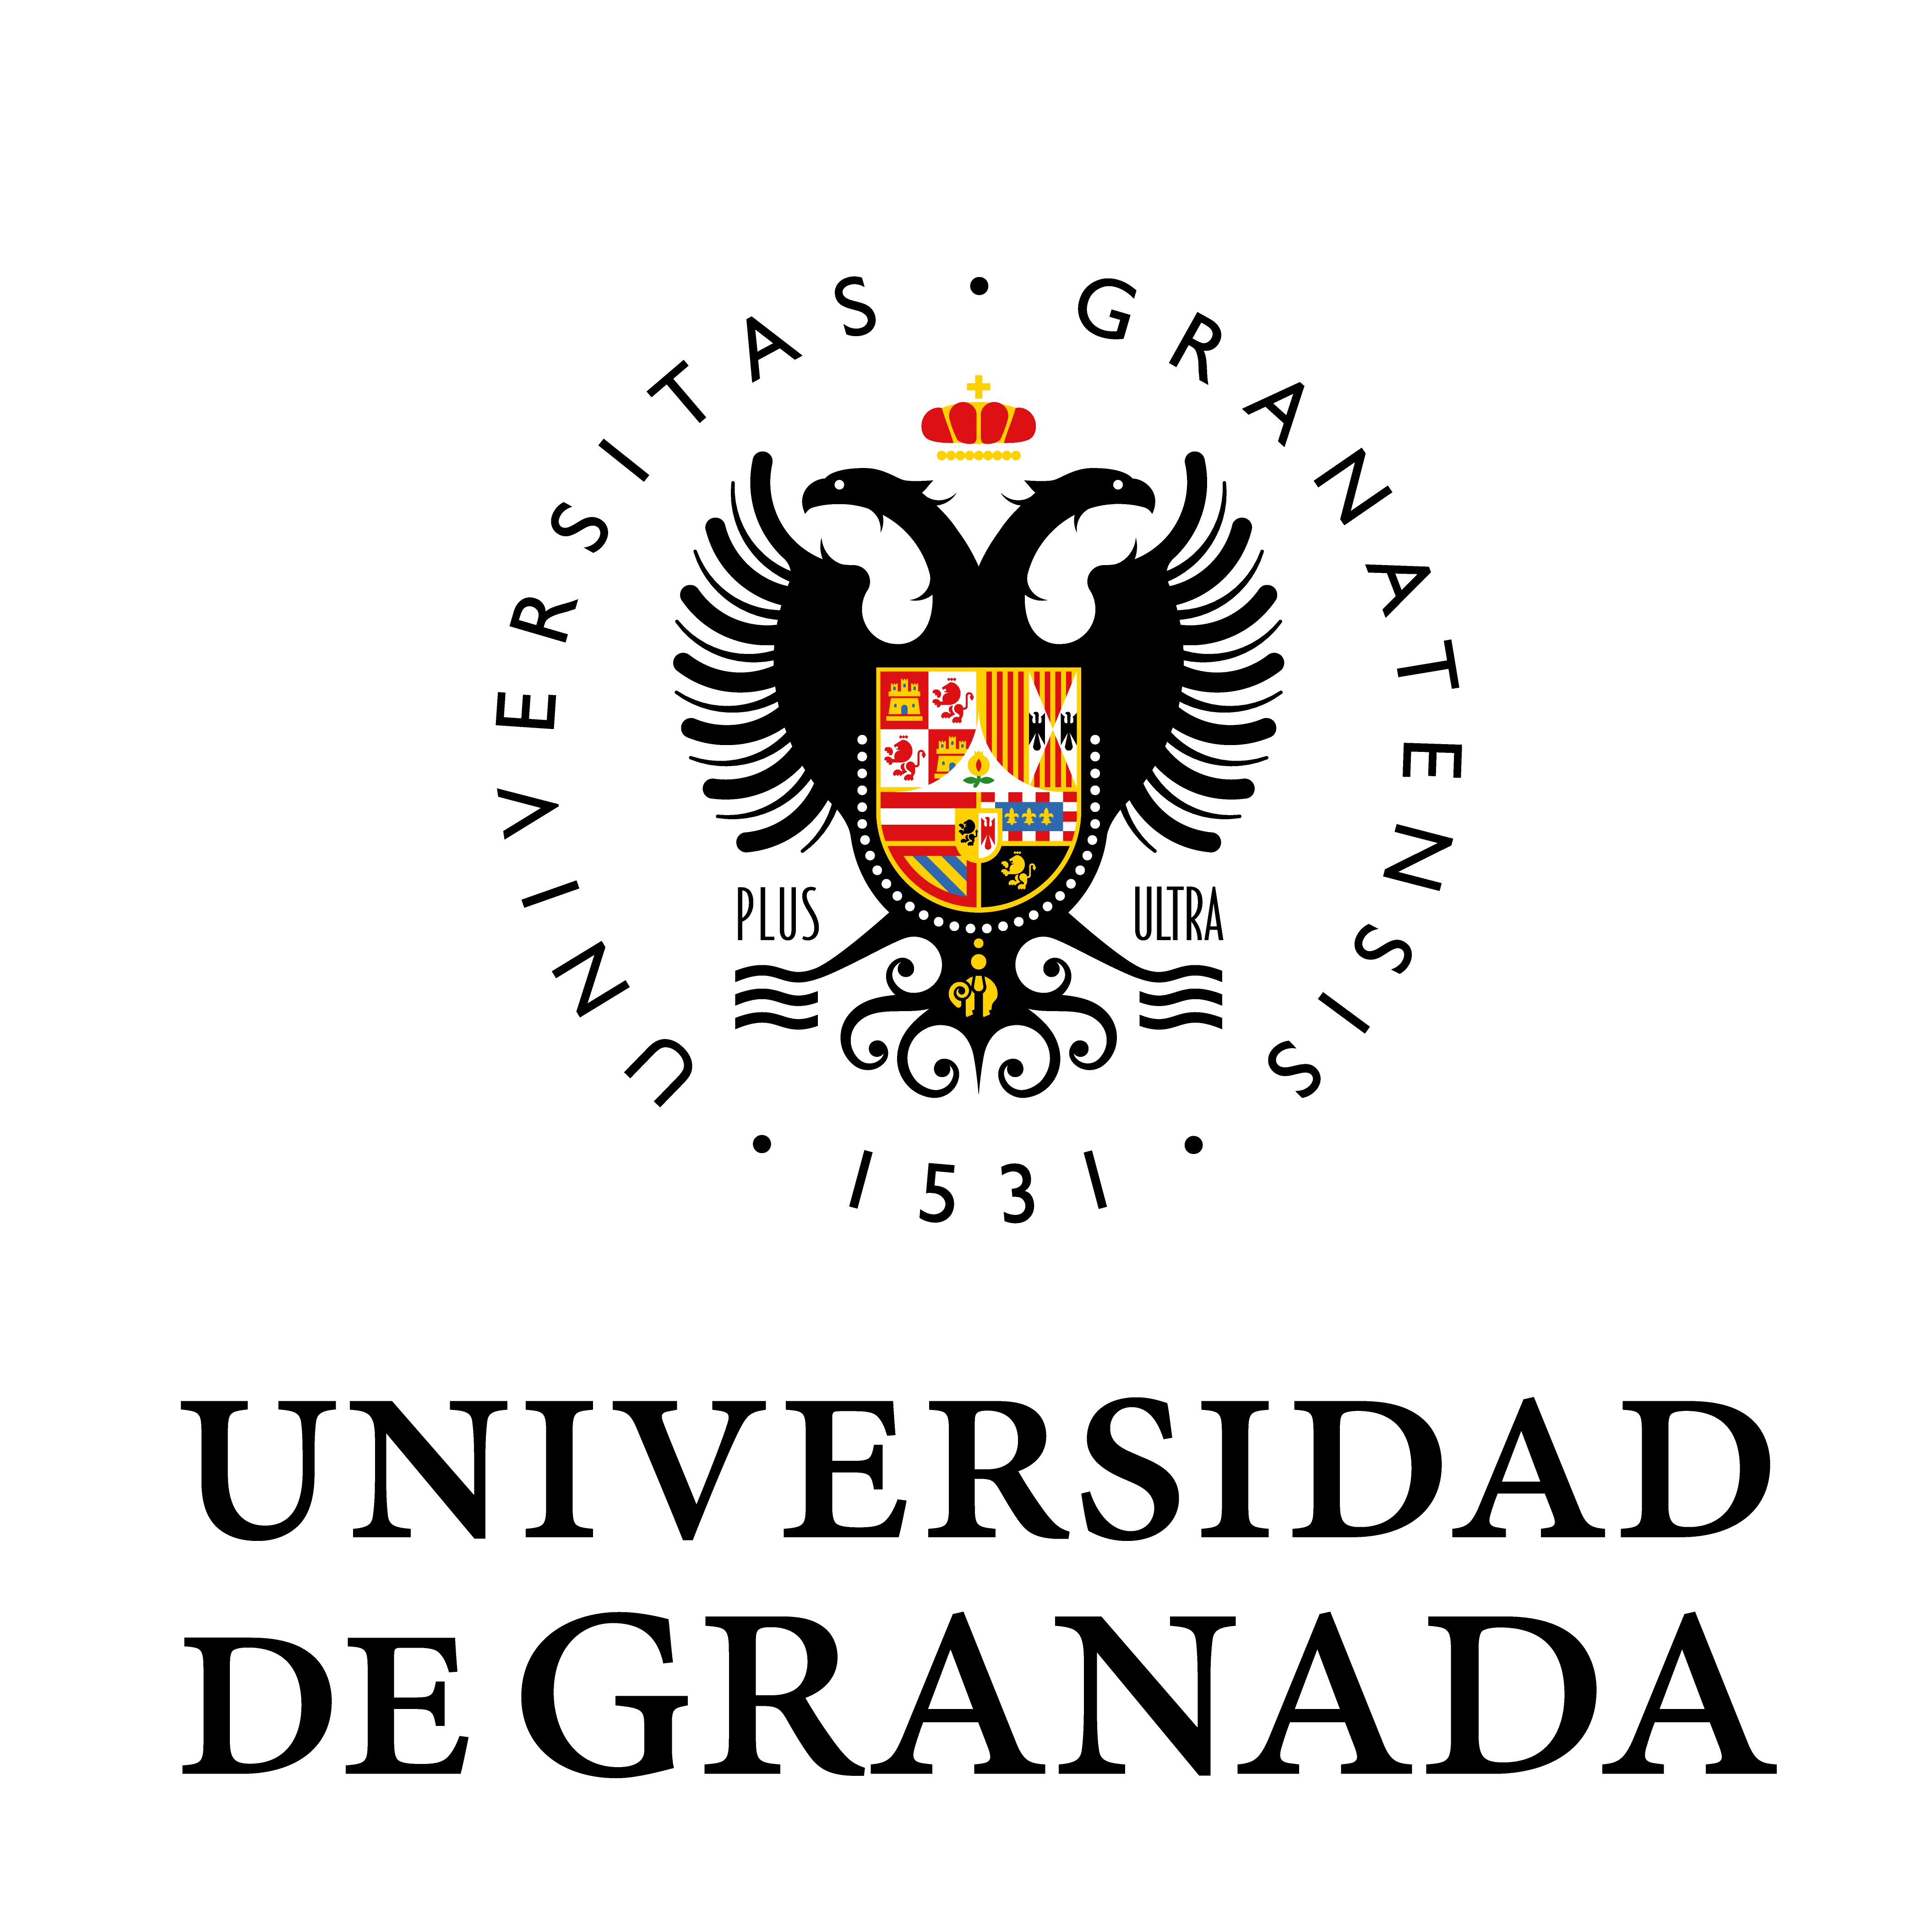
\includegraphics[width=0.35\textwidth]{escudo.png}\\[1.2cm]

    {\Huge\textbf{PROYECTO INDUSTRIAL}}\\[0.6em]

    {\LARGE\textbf{Ingeniería del Proyecto y Servicios Básicos}}\\[1.2em]

    {\LARGE\color{blue!75!black}\textbf{GRUPO 5: GESTIÓN DE SERVICIOS BÁSICOS}}\\[0.5em]

    {\Large\textbf{Estudio Técnico del Abastecimiento de Agua e Integración en Planta}}\\[1.5em]

}

\author{\Large\textbf{Christian Pérez Hita}\\[0.5em] \large Grado en Ingeniería Química \\ \large Universidad de Granada (UGR)}

\date{\today}



\begin{document}

\spanishdeactivate{.<>}

\setcounter{tocdepth}{3}

\maketitle



\newpage

\pdfbookmark[section]{\contentsname}{contenidos}

\tableofcontents

\newpage




%
% ==========================================================================
% CAPITULOS 1 AL 4 COMENTADOS TEMPORALMENTE (PRESERVADOS PARA CONSULTA)
% ==========================================================================

\chapter{Introducción y Objetivos del Trabajo}



\section{Objeto del Documento}

El presente trabajo técnico, enmarcado en el bloque de \textbf{Gestión de Servicios Básicos en la Ingeniería del Proyecto (Grupo 5)}, tiene como objetivo central el estudio integral, riguroso y multidisciplinar del abastecimiento de agua para una planta industrial de procesos químicos y biotecnológicos (tomando como caso de referencia la infraestructura de una biorrefinería y planta de bioproductos), contemplando su selección de fuentes, trámites legales de enganche, diseño y dimensionamiento hidráulico de la red interna, y un análisis exhaustivo de la \textbf{normativa sanitaria y medioambiental aplicable}.



El agua constituye uno de los suministros auxiliares (\textit{utilities}) más determinantes en cualquier complejo industrial moderno, desempeñando una multiplicidad de funciones vitales:

\begin{enumerate}

    \item \textbf{Agua de Proceso y Materia Prima:} Empleada en reactores químicos, fermentadores biotecnológicos, formulación de productos, lavado y extracción de biomasa.

    \item \textbf{Agua de Servicios Auxiliares Térmicos:} Fluido caloportador de refrigeración en condensadores y cambiadores de calor, así como agua de reposición y generación de vapor en calderas de vapor saturado.

    \item \textbf{Agua de Consumo Humano (AFCH y ACS):} Destinada al consumo directo de los operarios, servicios higiénicos, vestuarios, duchas y áreas de oficinas/laboratorios.

    \item \textbf{Agua Contra Incendios (PCI):} Reserva estricta y caudal presurizado para bocas de incendio equipadas (BIEs), rociadores y columnas hidrantes exteriores.

\end{enumerate}



\section{Estructura de Desarrollo}

El documento se articula en cuatro secciones principales de ingeniería:

\begin{itemize}

    \item \textbf{Capítulo 2: Captación desde Red Municipal de Abastecimiento:} Marco administrativo, requisitos técnicos de acometida, competencias locales y trámites con empresas concesionarias y ayuntamientos.

    \item \textbf{Capítulo 3: Captación Alternativa y Autoabastecimiento:} Análisis hidrogeológico e hidrológico de captaciones en pozos profundos, cursos superficiales (ríos) y embalses. Tramitación ante Confederaciones Hidrográficas.

    \item \textbf{Capítulo 4: Evaluación de Caudales y Dimensionamiento de la Red Interna:} Balances hídricos de proceso y consumos sanitarios, aplicación del CTE DB-HS 4, selección de materiales, cálculo de pérdidas de carga y dimensionamiento del grupo de presión y depósitos de acumulación.

    \item \textbf{Capítulo 5: Normativa Sanitaria y Medioambiental Aplicable:} Estudio profundo del Real Decreto 3/2023, prevención de \textit{Legionella} (RD 487/2022), Texto Refundido de la Ley de Aguas (RDL 1/2001), Reglamento del Dominio Público Hidráulico (RD 849/1986 y RD 665/2023), y Directiva Marco del Agua (Directiva 2000/60/CE).

\end{itemize}



%=============================================================================


\chapter{Captación desde Red Municipal: Requisitos, Marco Técnico y Trámites}
\label{cap:captacion_red_municipal}

\section{Marco General, Competencias y Modelos de Gestión Municipal}

De conformidad con el artículo 25.2 de la \textbf{Ley 7/1985, Reguladora de las Bases del Régimen Local (LRBRL)}, el abastecimiento domiciliario de agua potable a poblaciones y la evacuación y tratamiento de aguas residuales constituyen competencias propias, obligatorias e inexcusables de las entidades locales. Cuando un complejo fabril o planta de proceso biotecnológico y químico se implanta en suelo urbano consolidado o en un polígono industrial sectorizado, la conexión a la red de distribución municipal representa la alternativa técnica prioritaria por razones de seguridad de suministro, control bacteriológico continuo y garantía de caudal de origen.

La prestación del servicio público de distribución de agua y saneamiento puede articularse a través de tres modalidades jurídicas y operativas diferenciadas:
\begin{enumerate}
    \item \textbf{Gestión Directa Municipal:} Prestada por la propia administración local a través de sus servicios centrales o de una empresa pública de capital íntegramente municipal (p. ej., Aguas de Cádiz o EMASESA en determinados consorcios).
    \item \textbf{Gestión Indirecta por Concesión Administrativa Privada:} Formalizada mediante contrato de concesión demanial y explotación con operadores privados especializados (p. ej., Aqualia, Hidralia o Canal de Isabel II Gestión).
    \item \textbf{Empresa Mixta Público-Privada:} Modelo ampliamente consolidado en las principales capitales andaluzas, en el cual el capital social y los órganos de administración están compartidos entre la corporación municipal y el socio tecnológico privado. Un ejemplo representativo de esta figura es \textbf{EMASAGRA (Empresa Municipal de Abastecimiento y Saneamiento de Granada, S.A.)}, entidad responsable del ciclo integral del agua en la aglomeración urbana de Granada, participada mayoritariamente por el Excmo. Ayuntamiento de Granada junto al socio operador privado (\cite{EMASAGRA2026}).
\end{enumerate}

\section{Estimación Previa de Demandas y Consulta Cartográfica de Infraestructuras}

Con carácter preceptivo al inicio formal de cualquier expediente administrativo de enganche, el equipo de ingeniería debe determinar de manera rigurosa las magnitudes hidráulicas que definen la demanda de la planta:
\begin{itemize}
    \item \textbf{Caudal Medio Diario ($Q_{\text{md}}$):} Volumen total consumido en la factoría a lo largo de una jornada de trabajo ordinaria dividido por el tiempo efectivo de servicio, expresado en $\text{L/s}$ y $\text{m}^3/\text{día}$, desglosando los consumos propios del proceso químico, las reposiciones térmicas y las dotaciones de personal.
    \item \textbf{Caudal Punta Instantáneo Simultáneo ($Q_{\text{inst}}$):} Máxima demanda simultánea previsible en la cometida general ($\text{L/s}$), sobre la cual debe verificarse la capacidad portante de la red de distribución general sin que se induzcan depresiones inadmisibles en la malla urbana circundante.
    \item \textbf{Régimen Horario de Consumos y Factor de Carga:} Distribución de la curva de demanda horaria para evaluar el impacto de los consumos punta sobre la red general en horas de máxima solicitación comunitaria.
\end{itemize}

Para contrastar la viabilidad física del suministro y localizar los puntos óptimos de entronque, el proyectista dispone de sistemas de información geográfica e inventarios públicos de infraestructuras. En el ámbito territorial de la provincia de Granada, resulta de aplicación obligada la consulta a la plataforma de la \textbf{Encuesta de Infraestructura y Equipamientos Locales (EIEL)}, coordinada y gestionada por la \textbf{Diputación de Granada} (\cite{EIEL_Diputacion_Granada}).

La plataforma web de la EIEL permite al proyectista realizar la inspección geoespacial de la red de abastecimiento y saneamiento en el entorno de la parcela industrial:
\begin{enumerate}
    \item Identificación de las conducciones matrices que discurren por las calles limítrofes, consultando su material constructivo (fundición dúctil, polietileno de alta densidad PE 100 o fibrocemento en redes antiguas).
    \item Comprobación de diámetros nominales disponibles ($\text{DN }100\text{ mm}$, $\text{DN }150\text{ mm}$ o $\text{DN }200\text{ mm}$) y estado de conservación de la red.
    \item Localización de nudos de conexión, arquetas de sectorización, válvulas de compuerta y bocas de hidrante públicas adyacentes.
    \item Análisis de cotas topográficas de rasante y estimación preliminar de las presiones manométricas estáticas y dinámicas en el sector hidráulico correspondiente.
\end{enumerate}

\section{Requisitos Técnicos de la Acometida Industrial y Afección de Redes}

La acometida física es el conjunto de tuberías, piezas especiales y dispositivos que enlazan la canalización general municipal con la instalación general interior de la parcela. Sus requisitos de diseño se rigen por el \textit{Código Técnico de la Edificación (CTE DB-HS 4)} y las normas técnicas de la entidad gestora:

\begin{enumerate}
    \item \textbf{Presión de Servicio y Caudal Garantizado:}
          La empresa suministradora debe certificar mediante informe técnico vinculante las presiones de servicio en el nudo de entronque. De acuerdo con el CTE DB-HS 4:
          \begin{itemize}
              \item La presión manométrica estática no superará en ningún caso los $500\text{ kPa}$ ($50\text{ m.c.a.}$) para prevenir ruidos, golpes de ariete y roturas de mecanismos. Si la red municipal suministra una presión superior, se instalará obligatoriamente una válvula reductora de presión en cabecera.
              \item La presión manométrica dinámica mínima en los puntos terminales más desfavorables de la red interior no será inferior a $100\text{ kPa}$ ($10\text{ m.c.a.}$) para uso sanitario, y entre $200\text{ a }300\text{ kPa}$ ($20\text{ a }30\text{ m.c.a.}$) en tomas de proceso industrial y equipos contra incendios.
          \end{itemize}

    \item \textbf{Toma sobre Red General y Llave de Acometida:}
          La toma se realiza perpendicularmente a la canalización matriz mediante collarín de derivación en carga o te de fundición dúctil. En el límite exterior del dominio público se ubica la \textbf{llave de acometida}, alojada en arqueta normalizada con trampilla de fundición, accesible exclusivamente para el personal de la entidad suministradora.

    \item \textbf{Tubo de Alimentación y Armario de Contador General:}
          El tubo de alimentación enlaza la llave de acometida con la batería o armario general de contadores, discurriendo sin derivación intermedia alguna. El armario o arqueta general de contadores se sitúa en la linde de la parcela, en un paramento vertical accesible directamente desde el exterior, y aloja la siguiente valvulería y elementos de protección:
          \begin{itemize}
              \item \textbf{Válvula de corte general de entrada:} Llave de bola o compuerta elástica con orificio de purga manual.
              \item \textbf{Filtro en Y retenedor de sólidos:} Malla filtrante de acero inoxidable de $100\text{ }\mu\text{m}$ para retener arenas o partículas en suspensión procedentes de la red pública.
              \item \textbf{Contador general de agua homologado:} Equipo de medición volumétrico o electromagnético con homologación metrológica oficial, emisor de pulsos y módulo de telelectura vía radio.
              \item \textbf{Dispositivo de protección antirretorno (Desconector hidráulico):} Válvula de doble retención o desconector de zona de presión reducida no controlable (tipo BA, según UNE-EN 1717), que garantiza de forma física e inexorable que bajo ninguna circunstancia de sobrepresión interior o depresión de la red pueda retornar agua de proceso hacia la red pública de abastecimiento.
              \item \textbf{Válvula de corte de salida y grifo de toma de muestras:} Grifo sanitario dotado de purgador para el muestreo periódico y control analítico de la calidad bromatológica del agua suministrada, según exige el RD 3/2023.
          \end{itemize}

    \item \textbf{Cruces de Servicios y Distancias Reglamentarias en Zanja:}
          Las conducciones exteriores enterradas deben instalarse con una profundidad mínima de enterramiento de $0.80\text{ m}$ respecto a la rasante del terreno para amortiguar cargas mecánicas de tráfico pesado y prevenir heladas. En coexistencia con otras redes urbanas:
          \begin{itemize}
              \item La canalización de agua potable discurrirá siempre a una cota superior a la red de saneamiento de aguas residuales o pluviales, con una distancia vertical libre mínima de $0.30\text{ m}$ y una distancia horizontal mínima de $1.00\text{ m}$.
              \item Con respecto a cables eléctricos de baja o media tensión y canalizaciones de gas natural, se mantendrá una separación libre mínima de $0.50\text{ m}$.
          \end{itemize}
\end{enumerate}

\section{Procedimiento Administrativo, Modelo de Solicitud y Documentación Anexa}

El procedimiento técnico-administrativo para la obtención de la acometida de agua y saneamiento sigue un protocolo riguroso regulado por el Reglamento del Servicio de la entidad concesionaria y las Ordenanzas Municipales de Urbanismo (Figura~\ref{fig:tramites_red_municipal}).

\begin{figure}[H]
    \centering
    \adjustbox{max width=0.98\textwidth}{%
        \begin{tikzpicture}[>=Latex, node distance=1.1cm and 1.5cm, auto]
            \tikzstyle{block} = [rectangle, draw=blue!80!black, fill=blue!8, text width=4.0cm, text centered, rounded corners, minimum height=1.3cm, font=\small\bfseries]
            \tikzstyle{line} = [draw, -Latex, line width=1.2pt, blue!85!black]

            \node [block] (step1) {1. Solicitud de Viabilidad y Consulta Cartográfica (EIEL)};
            \node [block, right=of step1] (step2) {2. Redacción de Memoria Técnica de Acometida};
            \node [block, below=of step2] (step3) {3. Licencia de Obras Municipal (ICIO / Tasas)};
            \node [block, left=of step3] (step4) {4. Ejecución del Entronque e Inspección Técnica};
            \node [block, below=of step4] (step5) {5. Boletín de Fontanería, Contrato y Suministro};

            \path [line] (step1) -- node [above, font=\scriptsize] {Informe concesionaria} (step2);
            \path [line] (step2) -- node [right, font=\scriptsize] {Ingeniero Colegiado} (step3);
            \path [line] (step3) -- node [above, font=\scriptsize] {Apertura de zanjas} (step4);
            \path [line] (step4) -- node [left, font=\scriptsize] {Pruebas hidrostáticas} (step5);
        \end{tikzpicture}
    }
    \caption{Diagrama del iter administrativo para la formalización del suministro industrial municipal.}
    \label{fig:tramites_red_municipal}
\end{figure}

\subsection{Estructura del Formulario de Solicitud de Acometida (Modelo Oficial EMASAGRA)}

La solicitud formal de acometida de abastecimiento y vertido, formulada bajo el modelo oficial de EMASAGRA (\cite{EMASAGRA2026}), exige consignar exhaustivamente los siguientes bloques de datos:

\begin{enumerate}
    \item \textbf{Localización e Identificación Física de la Parcela:}
          \begin{itemize}
              \item Dirección exacta: Calle, número, código postal y término municipal.
              \item \textbf{Referencia Catastral Obligatoria:} Código alfanumérico de 20 dígitos asignado por la Dirección General del Catastro que individualiza unívocamente la finca rústica o urbana.
          \end{itemize}

    \item \textbf{Identificación Jurídica del Solicitante y Representación:}
          \begin{itemize}
              \item \textbf{Datos de la Sociedad Promotora:} Razón Social mercantil, Número de Identificación Fiscal (NIF) y domicilio social a efectos de notificaciones.
              \item \textbf{Representante Legal:} Persona física que ostenta poderes de representación mancomunados o solidarios en nombre de la sociedad, aportando su DNI/NIE y la escritura notarial de apoderamiento.
              \item \textbf{Delegado Técnico / Ingeniero Proyectista:} Técnico competente que actúa como interlocutor técnico ante los inspectores de la compañía concesionaria, consignando su nombre, titulación académica oficial, número de colegiado y Colegio Profesional correspondiente.
          \end{itemize}

    \item \textbf{Características Técnicas del Suministro Solicitado:}
          \begin{itemize}
              \item \textbf{Caudal punta simultáneo requerido ($\text{L/s}$):} Cuantificación del caudal máximo en la acometida para verificar la suficiencia hidráulica de la red municipal matriz.
              \item \textbf{Diámetro y Material de Acometida Propuesto:} Especificación del tubo de enlace exterior (típicamente polietileno PE 100 PN 16 de $\text{DN }63\text{ a }\text{DN }110\text{ mm}$, en función del balance de planta).
              \item \textbf{Tipología de Uso:} Declaración explícita de las actividades a suministrar (Consumo humano / Proceso industrial químico / Servicios auxiliares / Sistema de protección contra incendios).
          \end{itemize}

    \item \textbf{Datos del Vertido y Red de Saneamiento:}
          \begin{itemize}
              \item \textbf{Caudal punta de vertido ($\text{L/s}$):} Estimación del efluente máximo vertido tras su depuración en la estación depuradora de aguas residuales industriales (EDARI).
              \item \textbf{Cota de Acometida al Colector Municipal ($\text{m.s.n.m.}$):} Cota de solera de la tubería de saneamiento en el pozo de conexión público para asegurar la evacuación por gravedad o, en su defecto, justificar la estación de bombeo de efluentes (EBAR) de parcela.
          \end{itemize}
\end{enumerate}

\subsection{Relación Preceptiva de Documentación Anexa}

La solicitud formal debe acompañarse inexcusablemente de los siguientes documentos técnicos y jurídicos:
\begin{enumerate}
    \item \textbf{Licencia Municipal de Obras o Declaración Responsable Urbanística:} Copia autorizada del título habilitante expedido por la Gerencia de Urbanismo del Ayuntamiento correspondiente que autoriza la construcción o implantación de la actividad.
    \item \textbf{Plano de Situación y Parcela Acotado:} Cartografía georreferenciada a escala $1:500$ o $1:1000$ que sitúe la finca en la trama urbana con reflejo de sus lindes perimetrales y referencia catastral oficial.
    \item \textbf{Memoria Técnica de Abastecimiento y Saneamiento:} Documento técnico redactado y firmado por Ingeniero Colegiado competente que justifique los consumos diarios, caudales punta de simultaneidad, dimensionamiento de tuberías, cálculo de pérdidas de carga, características de los equipos y medidas de prevención contra la contaminación por reflujo (UNE-EN 1717).
    \item \textbf{Plano de Trazado de Acometida y Conexión Exterior:} Detalle acotado a escala $1:100$ o $1:200$ del entronque en la calzada, trazado de la tubería de alimentación, ubicación exacta de la llave de toma, arqueta de registro y armario de contador general según la normativa técnica municipal.
    \item \textbf{Acreditación Notarial de Representación Legal:} Copia de la escritura pública de constitución de la empresa promotora y poder de representación mercantil conferido a favor del solicitante.
\end{enumerate}

\chapter{Captación Alternativa: Pozos, Ríos y Embalses}



\section{Justificación Técnica y Económica del Autoabastecimiento}

En plantas industriales con consumos elevados de agua técnica (como biorrefinerías, plantas químicas o agroalimentarias donde el agua de proceso o refrigeración supera los $100\text{ m}^3/\text{día}$), la tarifa comercial municipal por metro cúbico puede condicionar gravemente la viabilidad económica del proyecto. El recurso a fuentes propias o alternativas representa una solución estratégica, supeditada a un régimen concesional riguroso:



\begin{table}[H]

    \centering

    \small

    \caption{Matriz comparativa de opciones de abastecimiento para complejos industriales}

    \label{tab:comparativa_fuentes}

    \begin{tabularx}{\textwidth}{@{}lXXXX@{}}

        \toprule

        \textbf{Criterio} & \textbf{Red Municipal} & \textbf{Pozo (Aguas Subterráneas)} & \textbf{Río (Aguas Superficiales)} & \textbf{Embalse / Canal de Riego} \\

        \midrule

        \textbf{Inversión Inicial ($CAPEX$)} & Muy baja (únicamente arqueta de acometida y contador). & Media-alta (sondeo, entubado, aforo y bomba sumergida). & Alta (obra de toma fluvial, desarenador y bombeo). & Media-alta (toma en canal y estación de impulsión). \\

        \addlinespace

        \textbf{Coste Operativo ($OPEX$)} & Muy elevado (tarifa municipal por bloque industrial). & Bajo (energía de bombeo y canon de control de vertidos). & Muy bajo (canon de regulación/utilización). & Reducido (canon hidrográfico y cuota de regantes). \\

        \addlinespace

        \textbf{Calidad Fisicoquímica} & Potable garantizada, desinfectada (RD 3/2023). & Estable térmicamente, pero con posible dureza y sales. & Variable con lluvias y turbidez (precisa clarificación). & Estable estacionalmente, pero con presencia de algas. \\

        \addlinespace

        \textbf{Garantía de Suministro} & Muy alta y continua (salvo averías en red general). & Elevada, supeditada al nivel piezométrico del acuífero. & Crítica en estiaje (condicionada al caudal ecológico). & Alta, planificada según calendarios de cuenca. \\

        \addlinespace

        \textbf{Complejidad Legal} & Baja (gestión municipal ordinaria de acometida). & Muy alta (Concesión C.H. y autorización de sondeos). & Muy alta (Concesión administrativa de dominio público). & Media-alta (concesión o convenio con Comunidad de Regantes). \\

        \bottomrule

    \end{tabularx}

\end{table}



\section{Captación Subterránea Mediante Pozos de Sondeo}

\begin{enumerate}

    \item \textbf{Estudio Hidrogeológico Previo:} Evaluación de la cuenca subterránea, litología, permeabilidad ($K$), transmisividad ($T$) y coeficiente de almacenamiento ($S$) del acuífero. Se ejecutan ensayos de bombeo escalonados (ensayos de aforo) para determinar la curva característica del pozo, el caudal específico ($Q/s$) y el cono de depresión generado para no agotar pozos colindantes.

    \item \textbf{Diseño Constructivo del Sondeo:}

    \begin{itemize}

        \item Perforación con lodo bentonítico o a rotopercución neumática.

        \item Entubado en acero al carbono o PVC ranurado (filtros de ranura continua Johnson en tramos acuíferos).

        \item Emparrillado de gravilla silícea seleccionada (\textit{gravel pack}) entre la perforación y la tubería para evitar el arrastre de finos y arenas a los rodetes de la bomba.

        \item Sellado cementado perimetral superior (mínimo los primeros $10\text{ m}$) para evitar la entrada de aguas pluviales superficiales contaminadas.

    \end{itemize}

    \item \textbf{Bomba Sumergible de Pozo Profundo:} Bomba centrífuga multietapa construida íntegramente en acero inoxidable AISI 304/316, accionada por motor eléctrico estanco con camisa de refrigeración y variador de frecuencia.

\end{enumerate}



\section{Captación Superficial en Ríos y Embalses}

\begin{enumerate}

    \item \textbf{Obras de Toma Fluvial:} Se ejecutan tomas laterales o pozos de ribera ranurados integrados en la margen. Deben dotarse de:

    \begin{itemize}

        \item Rejas de desbaste grueso y fino (limpieza manual o automática) con paso de luz inferior a $20\text{ mm}$ para impedir el paso de ramas, hojas y peces.

        \item Desarenadores de flujo laminar para sedimentar partículas abrasivas con velocidad de sedimentación superior a $0.2\text{ m/s}$.

    \end{itemize}

    \item \textbf{Condicionantes Hidrológicos en Estiaje:} Las extracciones fluviales están rígidamente subordinadas al mantenimiento del \textbf{caudal ecológico mínimo} fijado en los Planes Hidrológicos de Cuenca (artículo 42 del Texto Refundido de la Ley de Aguas). En períodos de sequía severa, la Confederación Hidrográfica tiene la potestad legal de clausurar o restringir unilateralmente las tomas industriales para priorizar el abastecimiento a poblaciones.



    Por ello, si una industria depende de tomas superficiales, es mandatorio proyectar \textbf{balsas de almacenamiento y regulación interna} capaces de dotar a la fábrica de una autonomía técnica de al menos $15\text{ a }30\text{ días}$ sin captación externa.

\end{enumerate}



\section{Trámites Concesionales ante el Organismo de Cuenca}

Todo aprovechamiento de aguas superficiales o subterráneas del Dominio Público Hidráulico requiere inexcusablemente el otorgamiento de una \textbf{Concesión Administrativa} por parte de la Confederación Hidrográfica competente (Guadalquivir, Segura, Ebro, Cuencas Mediterráneas Andaluzas, etc.) conforme al artículo 52 del TRLA:

\begin{itemize}

    \item \textbf{Petición y Proyecto Técnico de Concesión:} Memoria descriptiva, planos de la obra de toma, justificación estricta de las necesidades hídricas anuales ($\text{m}^3/\text{año}$) y caudal punta instantáneo ($\text{L/s}$).

    \item \textbf{Información Pública y Competencia de Proyectos:} Publicación en el Boletín Oficial del Estado (BOE) y Boletín Oficial de la Provincia (BOP) abriendo un plazo de 1 mes para presentación de alegaciones o proyectos en competencia.

    \item \textbf{Resolución Concesional:} Fija el volumen máximo anual autorizado, el caudal máximo instantáneo, el plazo de la concesión (máximo 75 años, habitualmente 20-25 años para actividades industriales), la obligación de instalar contadores homologados precintados con transmisión periódica de lecturas, y la liquidación periódica del \textbf{Canon de Utilización de las Aguas}.

\end{itemize}



%=============================================================================

\section{Captacion y Reutilizacion de Aguas Regeneradas (RD 1085/2024)}

\subsection{Paradigma de la Economia Circular del Agua en la Industria}

Frente a la creencia tradicional de que la regeneracion del agua es competencia exclusiva de las depuradoras publicas (EDAR) para vertido al rio o riego agricola, el reciente \textbf{Real Decreto 1085/2024, de 22 de octubre} (que deroga al antiguo RD 1620/2007 y transpone el Reglamento UE 2020/741) situa a las instalaciones industriales en el epicentro de la reutilizacion:

\begin{enumerate}

    \item \textbf{Doble Via de Reutilizacion en Planta:}

    \begin{itemize}

        \item \textbf{Reutilizacion Externa (Concesion de Agua Regenerada):} La industria suscribe un convenio o solicita concesion administrativa ante la Confederacion Hidrografica para captar directamente el efluente tratado en el tratamiento terciario de una EDAR municipal o comarcal vecina.

        \item \textbf{Reciclado Interno en Circuito Cerrado:} La propia planta implanta tratamientos de afino sobre sus efluentes o condensados limpios, recirculandolos a cabecera de procesos no sanitarios.

    \end{itemize}

    \item \textbf{Usos Industriales Autorizados y Prohibiciones Expresas:}

    El RD 1085/2024 establece una lista exhaustiva de 28 usos regulados agrupados por clases de calidad:

    \begin{itemize}

        \item \textbf{Usos Industriales Permitidos:} Aguas de refrigeracion en circuitos semicerrados (torres de refrigeracion y condensadores evaporativos, exigiendo riguroso control de \textit{Legionella}), aguas de alimentacion de calderas (previo desmineralizado), aguas de lavado de patios, viales y maquinaria pesada, y redes de extincion de incendios.

        \item \textbf{Prohibiciones Exclusivas:} Queda terminantemente prohibido el empleo de agua regenerada para el consumo humano directo, para la preparacion y procesado en la industria alimentaria o cosmetica cuando el agua entre en contacto intimo con el producto final (salvo que cumpla integramente los estandares de potabilidad del RD 3/2023), y en instalaciones hospitalarias.

    \end{itemize}

    \item \textbf{Plan de Gestion del Riesgo del Agua Regenerada (PGRAR):}

    Cualquier planta que utilice agua regenerada debe elaborar y someter a aprobacion de la Autoridad Sanitaria un PGRAR, analizando barreras multiples (desinfeccion UV, cloracion residual, filtros de cartucho), controles microbiologicos (ausencia de \textit{E. coli}, control de nematodos intestinales y turbidez inferior a 2 NTU) y protocolos de contingencia ante desviaciones.

\end{enumerate}






\chapter{Evaluación del Caudal Necesario y Dimensionamiento de la Red Interna}
\label{cap:caudal_dimensionamiento_red}

\section{Evaluación del Caudal Necesario y Balances Hídricos de Planta}

El diseño y dimensionamiento de la red hidráulica interior de una planta industrial de procesos químicos y biotecnológicos exige una evaluación cuantitativa exhaustiva y segregada de los diversos requerimientos de agua. De acuerdo con las buenas prácticas de ingeniería de proyectos y los estándares normativos (\cite{UNE_EN_806_3_2007, UNE_149201_2017}), deben cuantificarse tres tipos esenciales de caudales: el caudal medio diario, el caudal punta instantáneo simultáneo y la demanda de la red contra incendios.

\subsection{Caudal Medio Diario ($Q_{\text{md}}$) y Dotaciones de Consumo}

El caudal medio diario representa el consumo medio distribuido a lo largo del tiempo de operación de la planta:
\begin{equation}
    Q_{\text{md}} = \frac{V_{\text{diario total}}}{t_{\text{operación}}} \qquad \left[\frac{\text{L}}{\text{s}}\right]
    \label{eq:caudal_medio_diario}
\end{equation}
donde $V_{\text{diario total}}$ ($\text{m}^3$ o $\text{L}$) engloba la suma ponderada de las tres categorías funcionales de consumo del complejo industrial:

\begin{enumerate}
    \item \textbf{Consumo de Personal y Servicios Higiénico-Sanitarios:}
          Las dotaciones per cápita deben asignarse en función de las condiciones laborales y los perfiles de los puestos de trabajo:
          \begin{itemize}
              \item \textbf{Personal de oficinas, control y laboratorios (sin duchas):} Dotación reglamentaria de $30\text{ a }50\text{ L/persona}\cdot\text{día}$.
              \item \textbf{Personal operario de producción, mantenimiento y almacenes (con duchas y vestuarios):} Dotación industrial de $80\text{ a }120\text{ L/persona}\cdot\text{día}$, indispensable para cubrir las duchas de final de turno en ambientes químicos y el cumplimiento de las condiciones de seguridad y salud en el trabajo.
          \end{itemize}

    \item \textbf{Consumo de Proceso Industrial y Servicios Auxiliares Térmicos:}
          Estimado rigurosamente a partir de los balances de materia y energía de planta en régimen nominal continuo:
          \begin{itemize}
              \item \textbf{Circuito de Refrigeración Industrial:} Demanda de reposición hídrica en torres de refrigeración o condensadores barométricos para compensar las pérdidas por evaporación física ($E$), arrastre aerodinámico ($A$) y purgas continuas de salinidad ($P$), típicamente $1.5\text{ a }3.5\text{ L/s}$ para cargas térmicas moderadas ($\sim 300\text{ kW}$).
              \item \textbf{Generación de Vapor en Calderas Industriales:} Reposición de agua ablandada y desgasificada para compensar las purgas de lodos/sales ($5-10\%$) y las líneas de inyección directa de vapor vivo (esterilización, reactores de arrastre de biomasa o humidificación), con caudales en el rango de $0.20\text{ a }0.50\text{ L/s}$.
              \item \textbf{Agua de Reacción, Formulación y Extracción:} Agua de alta pureza incorporada directamente a fermentadores, tanques de disolución y síntesis química.
              \item \textbf{Sistemas de Limpieza CIP (\textit{Cleaning-In-Place}):} Lavado automático de reactores, centrífugas, conducciones y filtros prensa, con régimen discontinuo pero elevado consumo unitario ($1.5\text{ a }3.0\text{ L/s}$).
          \end{itemize}

    \item \textbf{Consumos de Servicios Exteriores y Mantenimiento de Parcela:}
          \begin{itemize}
              \item \textbf{Riego de zonas verdes y jardinería exterior:} Dotación estándar de $2\text{ a }4\text{ L/m}^2\cdot\text{día}$ durante el periodo estival.
              \item \textbf{Baldeo periódico de viales y soleras de carga/descarga:} Dotación de $1.5\text{ a }2.5\text{ L/m}^2\cdot\text{día}$ mediante tomas de manguera de alta presión.
          \end{itemize}
\end{enumerate}

\subsection{Caudal Punta Instantáneo Simultáneo de Diseño ($Q_{\text{inst}}$)}

El caudal de cálculo simultáneo determina el dimensionamiento de las tuberías generales de distribución, los grupos de sobrepresión y los equipos de pretratamiento. Los puntos de consumo higiénico no operan de forma continuada, por lo que su demanda simultánea se obtiene mediante el coeficiente de simultaneidad $K_s$ establecido en la norma UNE 149201 y en el CTE DB-HS 4 (\cite{CTE_DB_HS4, UNE_149201_2017}):
\begin{equation}
    K_s = \frac{1}{\sqrt{n - 1}} \qquad (n > 2)
    \label{eq:coef_simultaneidad}
\end{equation}
siendo $n$ el número total de aparatos sanitarios instalados en la factoría (inodoros, lavabos, duchas, urinarios, vertederos).

A partir de los caudales mínimos instantáneos fijados por la normativa para cada aparato (Tabla~\ref{tab:caudales_aparatos_norma}), el caudal simultáneo de diseño de la factoría se formula como:
\begin{equation}
    Q_{\text{inst}} = K_s \cdot \sum_{i=1}^{n} Q_{\text{aparato}, i} + Q_{\text{proceso, simultáneo}}
    \label{eq:caudal_punta_simultaneo}
\end{equation}
donde $Q_{\text{proceso, simultáneo}}$ representa la máxima suma simultánea de las demandas de proceso en régimen de punta operativa.

\begin{table}[H]
    \centering
    \small
    \renewcommand{\arraystretch}{1.20}
    \caption{Caudales instantáneos mínimos y presiones de servicio en aparatos (CTE DB-HS 4)}
    \label{tab:caudales_aparatos_norma}
    \begin{tabularx}{\textwidth}{@{}X c c c c@{}}
        \toprule
        \textbf{Tipo de Aparato Sanitario} & \textbf{Caudal AF (L/s)} & \textbf{Caudal ACS (L/s)} & \textbf{Presión (kPa)} & \textbf{Presión (m.c.a.)} \\
        \midrule
        Lavabo individual & $0.10$ & $0.065$ & $100$ & $10.0$ \\
        Inodoro con cisterna común & $0.10$ & -- & $100$ & $10.0$ \\
        Ducha colectiva de vestuarios & $0.20$ & $0.100$ & $100$ & $10.0$ \\
        Fregadero de laboratorio / comedor & $0.20$ & $0.100$ & $100$ & $10.0$ \\
        Vertedero de limpieza técnica & $0.20$ & -- & $100$ & $10.0$ \\
        Grifo de riego exterior ($\phi 20\text{ mm}$) & $0.40$ & -- & $100$ & $10.0$ \\
        Boca de baldeo industrial ($\phi 25\text{ mm}$) & $0.80$ & -- & $150$ & $15.0$ \\
        \bottomrule
    \end{tabularx}
\end{table}

\subsection{Caudal Específico del Sistema de Protección Contra Incendios (PCI)}

El agua para la red de protección contra incendios (PCI) está estrictamente regulada por el \textit{Reglamento de Seguridad Contra Incendios en Establecimientos Industriales (RSCIEI, RD 2267/2004)}, el \textit{Reglamento de Instalaciones de Protección Contra Incendios (RIPCI, RD 513/2017)}, la norma \textbf{UNE 23500:2021} sobre sistemas de abastecimiento de agua contra incendios y la norma \textbf{UNE-EN 12845:2016} para rociadores automáticos (\cite{RD_513_2017, UNE_23500_2021, UNE_EN_12845_2016}).

El caudal nominal requerido por la red de PCI se formula como:
\begin{equation}
    Q_{\text{PCI}} = Q_{\text{rociadores}} + Q_{\text{hidrantes/BIEs}}
    \label{eq:caudal_pci}
\end{equation}
Para un sector de incendio clasificado con nivel de riesgo intrínseco medio en planta química, los estándares de diseño fijan:
\begin{itemize}
    \item Bocas de Incendio Equipadas (BIEs de $\text{DN }25\text{ mm}$ o $\text{DN }45\text{ mm}$): Caudal mínimo de $1.6\text{ a }3.3\text{ L/s}$ por boca con presión residual mínima de $200\text{ kPa}$ ($20\text{ m.c.a.}$), con simultaneidad de funcionamiento de 2 bocas durante 60 minutos ($V_{\text{BIE}} \approx 12 - 24\text{ m}^3$).
    \item Hidrantes exteriores de columna húmeda ($\text{DN }100\text{ mm}$): Caudal mínimo de $16.6\text{ L/s}$ ($1000\text{ L/min}$) a $200\text{ kPa}$ durante 90 minutos ($V_{\text{hidrante}} \approx 90\text{ m}^3$).
    \item Rociadores automáticos: Densidad de aplicación entre $7.5\text{ y }12.5\text{ mm/min}$ sobre el área de operación de diseño según norma UNE-EN 12845.
\end{itemize}

Por mandato imperativo de la norma UNE 23500:2021, el volumen de agua asignado a la protección contra incendios es \textbf{exclusivo e inviolable}, no pudiendo ser compartido ni detraído por los consumos de proceso o sanitarios bajo ninguna condición de explotación.

\section{Diseño y Dimensionamiento de la Red Interna de Distribución}

\subsection{Depósito de Almacenamiento, Autonomía y Cámara de Rotura de Carga}

Para proteger el complejo industrial ante contingencias de desabastecimiento, averías en la red pública o variaciones acusadas de presión, se dispone un depósito de regulación y reserva dimensionado para garantizar una autonomía operativa de $24\text{ a }48\text{ horas}$:
\begin{equation}
    V_{\text{útil}} = Q_{\text{md}} \cdot t_{\text{autonomía}} \qquad \left[\text{m}^3\right]
    \label{eq:volumen_deposito}
\end{equation}

El diseño constructivo e hidráulico del depósito cumple dos requisitos técnicos fundamentales derivados de la normativa sanitaria y sectorial:
\begin{enumerate}
    \item \textbf{Depósito Partido en Dos Compartimentos Independientes:}
          De acuerdo con los criterios del RD 3/2023 y las pautas higiénico-sanitarias frente a \textit{Legionella} (RD 487/2022) (\cite{RD3_2023, RD487_2022}), el depósito no puede concebirse como un seno único indiviso. Se diseña obligatoriamente dividido en \textbf{dos compartimentos o vasos simétricos hidráulicamente independientes}, enlazados mediante un colector exterior de aspiración con valvulería de seccionamiento en bypass. Esta configuración permite aislar, vaciar, inspeccionar, limpiar y desinfectar periódicamente cualquiera de los vasos sin interrumpir en ningún momento el suministro continuo de agua a la planta.
    \item \textbf{Desconexión Hidráulica Atmosférica (Air Gap Break Tank):}
          En cumplimiento estricto de la norma \textbf{UNE-EN 1717} y el CTE DB-HS 4, la acometida municipal no puede conectarse de forma directa y presurizada a las líneas que alimentan los reactores químicos o las torres de enfriamiento. La alimentación municipal descarga en el depósito a través de una \textbf{cámara de aire de rotura de carga (separación atmosférica tipo AA/AB)}, donde la cota de salida de la tubería de llenado se sitúa a una distancia libre mínima superior a dos veces su diámetro por encima del labio superior de rebose del depósito. Esta discontinuidad física hace hidrodinámicamente imposible el retorno de fluidos por contrasifonado hacia la red pública de distribución.
\end{enumerate}

\subsection{Grupo de Presión (Estación de Sobreelevación) y Curva Resistente}

Dado que la descarga en el depósito se realiza a presión atmosférica, la red interior debe ser presurizada mediante un grupo de sobreelevación electromecánico. La altura manométrica total requerida por la bomba ($H_b$) se deduce a partir del balance energético en el punto hidráulico más desfavorable de la instalación:
\begin{equation}
    H_b = H_g + \Delta H + H_{\text{residual}} \qquad [\text{m.c.a.}]
    \label{eq:altura_manometrica_bomba}
\end{equation}
donde:
\begin{itemize}
    \item $H_g$ representa la altura geométrica entre la cota mínima de lámina de agua en el depósito y la cota de la toma terminal más elevada de la factoría ($\text{m}$).
    \item $\Delta H$ simboliza la pérdida de carga total acumulada (continua por fricción más singular por valvulería) a lo largo del tramo crítico hasta dicho punto ($\text{m.c.a.}$).
    \item $H_{\text{residual}}$ es la presión manométrica residual mínima de servicio exigida en el extremo de la toma:
          \begin{itemize}
              \item En aparatos sanitarios y griferías de vestuarios: $H_{\text{residual}} \ge 10 - 15\text{ m.c.a.}$ ($100 - 150\text{ kPa}$).
              \item En tomas de alimentación a intercambiadores, reactores y BIEs: $H_{\text{residual}} \ge 20 - 30\text{ m.c.a.}$ ($200 - 300\text{ kPa}$).
          \end{itemize}
\end{itemize}

El grupo de impulsión se estructura bajo una configuración \textbf{multi-bomba en paralelo ($2+1$ o $1+1$)} constituida por bombas centrífugas multietapa verticales de acero inoxidable AISI 316. La regulación de caudal se realiza mediante \textbf{variadores electrónicos de frecuencia (VFD)} integrados, los cuales adaptan la velocidad de giro de los rodetes a la demanda instantánea exacta de la planta, manteniendo una consigna de presión constante de $3.5\text{ a }4.0\text{ bar}$ en colector, con arranque progresivo sin picos de corriente y dotando al sistema de una bomba de reserva activa al $100\%$ de capacidad ante fallos mecánicos.

\subsection{Dimensionamiento Hidráulico de Tuberías y Criterios de Velocidad}

El cálculo del diámetro interior de cada tramo se efectúa aplicando la ecuación de continuidad a partir del caudal punta simultáneo transportado:
\begin{equation}
    Q = v \cdot \Omega = v \cdot \frac{\pi D_i^2}{4} \implies D_i = \sqrt{\frac{4 Q}{\pi \cdot v}}
    \label{eq:continuidad_diametro}
\end{equation}

El dimensionamiento impone límites de velocidad rigurosos para compatibilizar la amortiguación acústica, la prevención de la cavitación y la limitación de la sedimentación de biopelículas (\cite{SorianoRull2012}):
\begin{itemize}
    \item \textbf{Velocidad mínima autolimpiante ($v_{\text{mín}} = 0.5\text{ m/s}$):} Impuesta en toda la red de proceso y distribución general para evitar el estancamiento de fluidos, la sedimentación de partículas coloidales y la colonización microbiana.
    \item \textbf{Tuberías generales y colectores principales de planta:} Velocidad de flujo admisible de $v = 1.5\text{ a }2.0\text{ m/s}$.
    \item \textbf{Ramales de distribución secundaria y locales húmedos sanitarios:} Velocidad de flujo limitada a $v = 1.0\text{ a }1.2\text{ m/s}$ para prevenir ruidos molestos por fricción y fenómenos de corrosión-erosión en accesorios.
    \item \textbf{Red transitoria de protección contra incendios (PCI):} En situación excepcional de emergencia por siniestro, la velocidad puede elevarse hasta $v = 3.0\text{ a }4.0\text{ m/s}$ según norma UNE 23500.
\end{itemize}

Las pérdidas de carga continuas se cuantifican mediante la formulación fundamental de \textbf{Darcy-Weisbach}:
\begin{equation}
    h_f = f \cdot \frac{L}{D_i} \cdot \frac{v^2}{2g} \qquad [\text{m.c.a.}]
    \label{eq:darcy_weisbach}
\end{equation}
donde el factor de fricción adimensional $f$ se calcula con la ecuación universal de \textbf{Colebrook-White} para régimen turbulento en función de la rugosidad absoluta del material $\varepsilon$:
\begin{equation}
    \frac{1}{\sqrt{f}} = -2 \cdot \log_{10} \left( \frac{\varepsilon}{3.71 \cdot D_i} + \frac{2.51}{\text{Re} \cdot \sqrt{f}} \right)
    \label{eq:colebrook_white}
\end{equation}

Las pérdidas de carga localizadas o singulares generadas por codos, válvulas, tes y reducciones se evalúan mediante el método de los coeficientes de resistencia $K$:
\begin{equation}
    h_s = \sum_{j=1}^{m} K_j \cdot \frac{v^2}{2g} \qquad [\text{m.c.a.}]
    \label{eq:perdidas_singulares}
\end{equation}
o, de forma simplificada en fases de ingeniería básica, estimando una longitud equivalente acumulada del $20\text{ al }30\%$ de la longitud geométrica real del trazado ($L_{\text{eq}} = 1.20 - 1.30 L$).

\subsection{Selección Técnica de Materiales según Áreas Operativas}

La especificación de materiales debe responder a las exigencias de agresividad físico-química del suelo, presiones de trabajo, compatibilidad con agua de consumo humano según RD 3/2023 y resistencia térmica frente a desinfecciones:

\begin{enumerate}
    \item \textbf{Red Exterior Enterrada (Acometida y Distribución Perimetral):}
          Se prescribe \textbf{Polietileno de Alta Densidad (PE 100, clase PN 10 / PN 16, según UNE-EN 12201)}. Ofrece absoluta inmunidad frente a la corrosión galvánica y biológica de los suelos, elevada flexibilidad para admitir asentamientos diferenciales y ausencia de juntas mecánicas mediante uniones termosoldadas a tope o por manguito electrosoldable.
    \item \textbf{Red Interior de Edificación, Oficinas y Locales Húmedos (AFCH y ACS):}
          Se selecciona \textbf{Polipropileno Copolímero Random (PP-R, tipo 3, UNE-EN ISO 15874)} o tubería \textbf{multicapa (PE-RT/Al/PE-RT)}. Presentan nula rugosidad interna ($\varepsilon = 0.007\text{ mm}$), perfecta inercia bromatológica certificada en listas positivas para agua potable, baja conductividad térmica y resistencia certificada a desinfecciones térmicas periódicas a $70^\circ\text{C}$ frente a \textit{Legionella}.
    \item \textbf{Salas Técnicas de Proceso y Colectores Vistos de Planta:}
          Se prescribe \textbf{Acero Inoxidable Austenítico (AISI 304 o AISI 316L, UNE-EN 10217-7)}. Proporciona alta resistencia estructural a presiones elevadas, choques térmicos, vapor limpio y agentes desinfectantes oxidantes (ozono y dióxido de cloro), permitiendo el montaje modular mediante uniones ranuradas tipo \textit{Victaulic} o soldadura TIG con purga interior de gas inerte.
    \item \textbf{Red Específica Contra Incendios (PCI):}
          Tubería de \textbf{acero al carbono galvanizado en caliente (UNE-EN 10255)} sin soldadura o con costura longitudinal ensayada para clase de presión de diseño no inferior a $16\text{ bar}$.
\end{enumerate}

\subsection{Dispositivos Hidráulicos de Protección, Seguridad y Control}

La red se complementa con dispositivos específicos de control hidráulico:
\begin{itemize}
    \item \textbf{Válvulas Reductoras de Presión (PRV):} Instaladas en los ramales interiores siempre que la presión estática o dinámica sobrepase los $500\text{ kPa}$ ($50\text{ m.c.a.}$) para proteger griferías y juntas de estanqueidad.
    \item \textbf{Vasos de Expansión Hidroneumáticos (Calderines de Membrana):} Depósitos cerrados de acero con membrana de butilo alimentario y colchón de nitrógeno a contrapresión, dimensionados para absorber la onda elástica del \textbf{golpe de ariete} generada por el cierre rápido de electroválvulas de proceso (cálculo de la celeridad $c$ según fórmula de Joukowsky) y reducir la frecuencia horaria de arranque de las bombas principales.
    \item \textbf{Válvulas de Retención de Doble Disco Guiado:} A la impulsión de cada bomba y en ramales de proceso para impedir inversiones de flujo.
    \item \textbf{Ventosas Automáticas Trifuncionales:} Ubicadas en los puntos topográficos altos de los colectores para evacuar aire durante el llenado de la red, purgar microburbujas en régimen continuo y admitir aire atmosférico en caso de vaciado súbito para evitar depresiones de colapso.
    \item \textbf{Válvulas de Purga y Desagüe:} Dispuestas en los puntos bajos de las conducciones con arqueta conectada a la red de vertidos para permitir el vaciado completo de tramos en operaciones de mantenimiento o descontaminación.
\end{itemize}

\section{Trenes de Pretratamiento y Afino de Agua según Uso en Planta}

El agua captada de la red municipal presenta calidad potable garantizada para consumo humano, pero sus características fisicoquímicas pueden requerir tratamientos complementarios de adecuación para su empleo en procesos industriales específicos:
\begin{enumerate}
    \item \textbf{Descalcificación por Intercambio Iónico:} Filtración a través de resinas catiónicas de ciclo sodio para reducir la dureza total del agua a $< 5\text{ mg/L de CaCO}_3$ en la alimentación de calderas y circuitos de condensados, previniendo incrustaciones calcáreas de alta resistencia térmica.
    \item \textbf{Desmineralización Avanzada por Ósmosis Inversa (RO):} Reducción de la conductividad eléctrica a $< 10\text{ }\mu\text{S/cm}$ mediante membranas poliamídicas semipermeables para la formulación de medios biotecnológicos de fermentación y agua purificada de laboratorio.
    \item \textbf{Filtración por Carbón Activo Granular (CAG) y Cartuchos:} Retención del cloro residual libre para evitar el envenenamiento de catalizadores o la degradación de membranas poliméricas, completada con cartuchos absolutos de $0.2\text{ }\mu\text{m}$ en líneas estériles.
    \item \textbf{Dosificación Controlada de Biocida Oxidante Residual:} Mantenimiento de una concentración de cloro libre residual entre $0.2\text{ y }1.0\text{ mg/L}$ o dióxido de cloro en el depósito de acumulación general para garantizar la barrera desinfectante preventiva contra biopelículas en cumplimiento del RD 3/2023.
\end{enumerate}

\section[Digitalización y Telemetría Hídrica (Orden TED/339/2023)]{Digitalización, Telemetría y Contabilidad Hídrica (Orden TED/339/2023)}

En concordancia con la \textbf{Orden TED/339/2023}, la instalación incorpora un sistema integral de contabilidad hídrica y telemedida digital enlazado al sistema SCADA central de la factoría. Se instalan caudalímetros electromagnéticos divisionarios en la entrada de la acometida, la alimentación a calderas, las torres de refrigeración, las líneas de proceso y los consumos de personal. La monitorización en tiempo real permite detectar precozmente fugas internas, calcular los indicadores de intensidad hídrica por tonelada de producto fabricado y verificar de manera continua el balance hídrico global de la planta.



\chapter{Normativa Sanitaria, Medioambiental y Red de Saneamiento Industrial}

El abastecimiento de agua y la evacuación de efluentes en un complejo de ingeniería química o planta de proceso industrial están sujetos a un régimen regulatorio multidisciplinar y jerárquico. La viabilidad técnica y legal del proyecto depende del cumplimiento sincrónico de la legislación higiénico-sanitaria para agua de consumo y procesos limpios, los reglamentos de seguridad industrial contra riesgos biológicos (\textit{Legionella}), la normativa medioambiental sobre vertidos y protección de masas receptoras (aguas subterráneas y superficiales) y los códigos constructivos y de diseño que rigen las redes de evacuación y saneamiento (\cite{TRLA2001, RDPH1986, RD3_2023, RD487_2022, UNE_EN_752, CTE_DB_HS5, UNE_EN_ISO_129_1, ISO_4067_1, ISO_4067_6}).

\begin{figure}[htbp]
\centering
\begin{tikzpicture}[node distance=1.3cm, auto,
    bloque/.style={rectangle, draw=blue!70!black, fill=blue!5, rounded corners=3pt, thick, text width=4.0cm, align=center, minimum height=1.0cm, font=\small},
    norma/.style={rectangle, draw=teal!80!black, fill=teal!10, rounded corners=3pt, dashed, thick, text width=4.2cm, align=center, minimum height=1.0cm, font=\footnotesize},
    linea/.style={draw=gray!80!black, -{Latex[length=2.5mm]}, thick}]
    
    \node [bloque] (origen) {\textbf{Captación \& Red Municipal}\\Abastecimiento industrial};
    \node [norma, right=1.6cm of origen] (n1) {\textbf{RD 3/2023} (Consumo/Proceso)\\Lista positiva de materiales};
    
    \node [bloque, below=0.9cm of origen] (uso) {\textbf{Distribución \& Torres}\\Procesos y refrigeración};
    \node [norma, right=1.6cm of uso] (n2) {\textbf{RD 487/2022} (Legionelosis)\\PPCL / PSL y biocidas};
    
    \node [bloque, below=0.9cm of uso] (red) {\textbf{Red de Saneamiento Interna}\\Redes separativas y arquetas};
    \node [norma, right=1.6cm of red] (n3) {\textbf{CTE DB-HS 5 / UNE-EN 752}\\UNE-EN ISO 129-1 (dibujo)};
    
    \node [bloque, below=0.9cm of red] (vertido) {\textbf{EDARI \& Evacuación Final}\\Colector público o DPH};
    \node [norma, right=1.6cm of vertido] (n4) {\textbf{TRLA / RD 665/2023 / Dir. 2024/3019}\\Canon vertido y VLE};
    
    \path [linea] (origen) -- (uso);
    \path [linea] (uso) -- (red);
    \path [linea] (red) -- (vertido);
    
    \draw [dashed, draw=gray!70, thick] (origen) -- (n1);
    \draw [dashed, draw=gray!70, thick] (uso) -- (n2);
    \draw [dashed, draw=gray!70, thick] (red) -- (n3);
    \draw [dashed, draw=gray!70, thick] (vertido) -- (n4);
\end{tikzpicture}
\caption{Estructura regulatoria integral aplicable al ciclo del agua y saneamiento en plantas químicas e industriales.}
\label{fig:mapa_normativo_integral}
\end{figure}

\section{Marco Jurídico Integrado del Agua en España}

El marco regulatorio hidráulico e higiénico español se estructura en torno a tres pilares coordinados:
\begin{enumerate}
    \item \textbf{Gestión de la Oferta y Calidad de Captación:} Regido por el Texto Refundido de la Ley de Aguas (\cite{TRLA2001}) y su reglamento instrumental, el Reglamento del Dominio Público Hidráulico (\cite{RDPH1986}), recientemente modernizado mediante el \textbf{Real Decreto 665/2023}.
    \item \textbf{Seguridad Sanitaria en Instalaciones Interiores y Usos Especiales:} Articulado por el \textbf{Real Decreto 3/2023} (\cite{RD3_2023}) sobre aguas de consumo y materiales en contacto, junto con el \textbf{Real Decreto 487/2022} y el \textbf{Real Decreto 614/2024} (\cite{RD487_2022, RD614_2024}) de prevención higiénico-sanitaria de la legionelosis en equipos evaporativos e intercambiadores.
    \item \textbf{Economía Circular, Evacuación de Efluentes y Redes de Saneamiento:} Regido a nivel europeo por la nueva \textbf{Directiva (UE) 2024/3019} (\cite{DirectivaUE_2024_3019}), y a nivel técnico-constructivo y de delineación de planos por el Código Técnico de la Edificación (\cite{CTE_DB_HS5}), la norma europea de alcantarillado exterior e industrial \textbf{UNE-EN 752} (\cite{UNE_EN_752}, actualmente en revisión bajo el proyecto de enmienda \textbf{PNE-EN 752:2017/prA1} para adaptación a eventos climáticos extremos), las directrices vigentes de acotación \textbf{UNE-EN ISO 129-1:2019} (\cite{UNE_EN_ISO_129_1}) (sin que exista una norma única vigente de símbolos de arquetas y pozos, ver sección~\ref{sec:planos_reales}).
\end{enumerate}

\section{Normativa Sanitaria de Calidad del Agua}

\subsection{Real Decreto 3/2023: Criterios Técnico-Sanitarios del Agua de Consumo e Industrial}
El \textbf{Real Decreto 3/2023}, de 10 de enero, transpone la Directiva (UE) 2020/2184, estableciendo un nuevo paradigma de aseguramiento de calidad basado en planes de evaluación del riesgo (\textit{Water Safety Plans}):
\begin{itemize}
    \item \textbf{Lista Positiva de Materiales en Contacto:} El RD 3/2023 impide instalar tuberías, racores, juntas, valvulería o recubrimientos epóxicos que liberen sustancias nocivas o alteren las propiedades organolépticas del agua. En proyectos químicos, las líneas que sirvan como base para preparación de reactivos, calderas de vapor limpio, laboratorios o aseos deben justificar certificados de conformidad sanitaria.
    \item \textbf{Protección contra Retorno y Dispositivos Antirretorno:} El diseño de la red interna de abastecimiento debe impedir físicamente cualquier retorno o sifonamiento de fluidos de proceso hacia la red de distribución general, instalando desconectores hidráulicos de zona de presión reducida no comprobable o comprobable tipo BA (\cite{CTE_DB_HS4}).
    \item \textbf{Valores paramétricos:} El anexo I del RD 3/2023 fija valores para metales (plomo, níquel, cromo, etc.), subproductos de desinfección (trihalometanos $\le 100\,\mu\text{g/L}$) y desinfectante residual en red (cloro libre entre $0.2$ y $1.0\,\text{mg/L}$); las cifras exactas y sus plazos de aplicación deben tomarse del texto consolidado (\cite{RD3_2023}).
\end{itemize}

\subsection{Prevención y Control de la Legionelosis: RD 487/2022 y su Modificación por el Real Decreto 614/2024}
En la industria química y de procesos, los sistemas de refrigeración evaporativa (torres de refrigeración, condensadores evaporativos, aeroenfriadores adiabáticos) y las redes de agua caliente sanitaria (ACS) e industrial constituyen instalaciones de alto riesgo de proliferación y aerosolización de \textit{Legionella pneumophila}. El régimen legal se articula en el marco base del \textbf{Real Decreto 487/2022}, recientemente actualizado y precisado por el \textbf{Real Decreto 614/2024} (\cite{RD487_2022, RD614_2024}):

\begin{itemize}
    \item \textbf{Delimitación de Responsabilidad (Titular y Persona Explotadora):} El RD 614/2024 clarifica que cuando la explotación de las instalaciones industriales o auxiliares se encomiende a un tercero (gestor o empresa operadora), la responsabilidad legal del cumplimiento sanitario y documental recae directamente sobre la \textbf{persona física o jurídica explotadora}, salvo cláusula contractual fehaciente en contrario.
    \item \textbf{Planes de Gestión del Riesgo (PPCL vs. PSL):} La instalación debe operar bajo una de las dos figuras reconocidas:
    \begin{itemize}
        \item \textbf{Plan de Prevención y Control de Legionella (PPCL):} Basado en programas preestablecidos de mantenimiento, purgas por conductividad, dosificación continua de biocidas autorizados (ROESB) y limpiezas semestrales.
        \item \textbf{Plan Sanitario de Legionella (PSL):} Basado en la metodología de evaluación cuantitativa del riesgo de la OMS, adaptable a las particularidades de procesos industriales continuos.
    \end{itemize}
    \item \textbf{Toma de Muestras y Acreditación UNE-EN ISO/IEC 17025:} El RD 614/2024 exige formalmente que la toma de muestras de agua para análisis de \textit{Legionella} sea ejecutada por entidades acreditadas conforme a la norma UNE-EN ISO/IEC 17025:2017 (con plazo transitorio de acreditación hasta el 1 de enero de 2030).
    \item \textbf{Eficiencia Hídrica y Flexibilización de Vaciados:} El RD 614/2024 suprime la obligación sistemática de vaciado total en grandes sistemas y circuitos de refrigeración continuos durante las labores de limpieza y desinfección, permitiendo la recirculación controlada del agua para evitar el despilfarro masivo de recurso hídrico, siempre que se garantice la eficacia biocida.
    \item \textbf{Acciones Correctoras según Resultados Analíticos en Torres de Refrigeración (Anexo VIII, Tabla 8):} Las actuaciones obligatorias ante recuentos de \textit{Legionella spp.} en torres y condensadores evaporativos (actualizadas por el RD 614/2024) son:
    \begin{itemize}
        \item \textbf{No detectado o $< 100\,\text{UFC/L}$:} Mantener las condiciones normales de operación y tratamiento.
        \item \textbf{$\ge 100$ y $< 1\,000\,\text{UFC/L}$:} Revisar de inmediato el programa de tratamiento de agua y dosificación biocida, realizar las correcciones oportunas y \textbf{valorar técnicamente efectuar una limpieza y desinfección} (matiz de ponderación técnica introducido por el RD 614/2024), con remuestreo de comprobación a los 15--30 días.
        \item \textbf{$\ge 1\,000$ y $< 10\,000\,\text{UFC/L}$:} Es \textbf{obligatorio} realizar una limpieza y choque de desinfección química de todo el circuito, revisar exhaustivamente los parámetros físico-químicos (biocida libre, pH, purga) y tomar muestra de control a los 15--30 días.
        \item \textbf{$\ge 10\,000\,\text{UFC/L}$:} Supone riesgo higiénico inaceptable: \textbf{parada cautelar e inmediata de la instalación}, ejecución de limpieza de choque y desinfección exhaustiva, y remuestreo reglamentario antes de reanudar el servicio ordinario.
    \end{itemize}
\end{itemize}

\section{Redes de Saneamiento Industrial y Evacuación de Efluentes}

El diseño de la red de saneamiento en un proyecto de ingeniería química no se limita a un mero desagüe, sino que constituye una infraestructura crítica de seguridad ambiental, contención de fugas y cumplimiento legal (\cite{UNE_EN_752, CTE_DB_HS5}).

\subsection{Topología Separativa Estricta en Plantas Químicas}
A diferencia de los edificios residenciales, una instalación industrial de proceso requiere la segregación física e hidráulica en un mínimo de cuatro subredes independientes:
\begin{enumerate}
    \item \textbf{Red de Fecales o Aguas Negras (R-FEC):} Procedente de vestuarios, comedores y aseos del personal. Se conduce directamente hacia la arqueta sifónica general de acometida al colector municipal, sin mezclarse previamente con efluentes de fabricación.
    \item \textbf{Red de Pluviales Limpias (R-PLU):} Recoge escorrentías de cubiertas de naves y viales perimetrales limpios sin riesgo de derrame químico. Puede conducirse a balsas de laminación o vertido directo a cauce/red municipal sin tratamiento previo intensivo.
    \item \textbf{Red de Pluviales Potencialmente Contaminadas (R-PLC):} Aguas de lluvia caídas sobre zonas de carga/descarga de cisternas, parques de tanques, áreas de proceso exterior y muelles. Obligatoriamente canalizadas hacia un sistema de retención de las primeras lluvias (primeros $15\text{--}20\,\text{mm}$ de precipitación) y enviadas a desarenador y \textbf{separador de hidrocarburos / decantador}.
    \item \textbf{Red de Vertidos Industriales de Proceso (R-IND):} Aguas procedentes de purgas de calderas, rechazos de ósmosis inversa, limpiezas CIP (\textit{Cleaning-in-Place}), condensados contaminados y condensadores barométricos. Estas aguas se canalizan mediante tuberías químicamente resistentes hacia la estación depuradora de aguas residuales industriales (\textbf{EDARI}) para su neutralización, coagulación-floculación y tratamiento biológico/químico antes de su vertido o reutilización.
\end{enumerate}

\begin{figure}[htbp]
\centering
\begin{tikzpicture}[node distance=1.1cm, auto,
    % Estilos clasificados por tipo de efluente (concordantes con Tabla 5.1)
    caja_plu/.style={rectangle, draw=blue!80!black, fill=blue!10, rounded corners=2pt, thick, text width=2.9cm, align=center, minimum height=0.9cm, font=\scriptsize},
    caja_plc/.style={rectangle, draw=blue!75!cyan, fill=cyan!10, rounded corners=2pt, thick, text width=2.9cm, align=center, minimum height=0.9cm, font=\scriptsize},
    caja_fec/.style={rectangle, draw=red!80!black, fill=red!10, rounded corners=2pt, thick, text width=2.9cm, align=center, minimum height=0.9cm, font=\scriptsize},
    caja_ind/.style={rectangle, draw=green!50!black, fill=green!10, rounded corners=2pt, thick, text width=2.9cm, align=center, minimum height=0.9cm, font=\scriptsize},
    pozo/.style={rectangle, draw=magenta!80!black, fill=magenta!15, thick, rounded corners=3pt, text width=2.8cm, align=center, minimum height=0.9cm, font=\scriptsize},
    ptm/.style={rectangle, draw=black!85, fill=gray!15, thick, rounded corners=3pt, text width=2.8cm, align=center, minimum height=0.9cm, font=\scriptsize},
    destino/.style={rectangle, draw=teal!90!black, fill=teal!20, rounded corners=4pt, line width=1.1pt, text width=3.2cm, align=center, minimum height=1.0cm, font=\small\bfseries},
    flecha_plu/.style={draw=blue!80!black, -{Latex[length=2.3mm]}, thick},
    flecha_plc/.style={draw=blue!75!cyan, -{Latex[length=2.3mm]}, thick, dashed},
    flecha_fec/.style={draw=red!80!black, -{Latex[length=2.3mm]}, thick},
    flecha_ind/.style={draw=green!50!black, -{Latex[length=2.3mm]}, thick},
    flecha_gen/.style={draw=gray!80!black, -{Latex[length=2.3mm]}, thick}]
    
    % Unidades de origen
    \node [caja_plu] (cubiertas) {\textbf{Cubiertas Naves}\\(Pluviales limpias)};
    \node [caja_plc, below=0.6cm of cubiertas] (viales) {\textbf{Zonas Carga / Viales}\\(Pluviales contam.)};
    \node [caja_fec, below=0.6cm of viales] (edif) {\textbf{Edificio Servicios}\\(Aguas fecales)};
    \node [caja_ind, below=0.6cm of edif] (proceso) {\textbf{Reactores / CIP / Purga}\\(Vertido industrial)};
    
    % Elementos intermedios y tratamiento
    \node [caja_plu, right=1.2cm of cubiertas] (arc_plu) {Arqueta de Paso\\(\textbf{R-PLU})};
    \node [caja_plc, right=1.2cm of viales] (sep_hid) {Separador de\\Hidrocarburos (\textbf{SH})};
    \node [caja_fec, right=1.2cm of edif] (arc_sif) {Arqueta Sifónica\\(\textbf{R-FEC})};
    \node [caja_ind, right=1.2cm of proceso] (edari) {EDARI Planta\\(\textbf{R-IND}: Neutraliz. + F-Q)};
    
    % Colector general y pozo de control
    \node [pozo, right=1.3cm of sep_hid] (pozo_unif) {\textbf{Pozo de Registro (PR)}\\General de Pluviales};
    \node [ptm, right=1.3cm of edari] (pozo_muestras) {\textbf{Pozo Homologado (PTM)}\\Toma de Muestras Oficial};
    
    % Destino final
    \node [destino, right=1.2cm of pozo_unif, yshift=-1.1cm] (emisor) {Colector Municipal o\\Cauce Receptor (DPH)};
    
    % Conexiones diferenciadas por efluente
    \path [flecha_plu] (cubiertas) -- (arc_plu);
    \path [flecha_plc] (viales) -- (sep_hid);
    \path [flecha_fec] (edif) -- (arc_sif);
    \path [flecha_ind] (proceso) -- (edari);
    
    \path [flecha_plu] (arc_plu) -| (pozo_unif);
    \path [flecha_plc] (sep_hid) -- (pozo_unif);
    \path [flecha_fec] (arc_sif) -| (pozo_muestras);
    \path [flecha_ind] (edari) -- (pozo_muestras);
    
    \path [flecha_plu] (pozo_unif) -- (emisor);
    \path [flecha_gen] (pozo_muestras) -- (emisor);
\end{tikzpicture}
\caption{Diagrama de bloques de la red separativa de saneamiento y tratamiento previo en un complejo de ingeniería química (código de colores concordante con la simbología de la Tabla~\ref{tab:simbologia_saneamiento}).}
\label{fig:diagrama_saneamiento_quimico}
\end{figure}

\subsection{Elementos Singulares de la Red de Evacuación}
Conforme a las prescripciones del CTE DB-HS 5 y la UNE-EN 752, toda red industrial debe estructurarse con los siguientes componentes normalizados:
\begin{itemize}
    \item \textbf{Arquetas a Pie de Bajante (APB):} Recogen las aguas verticales de bajantes pluviales o fecales con registro roscado hermético para desobstrucción, evitando uniones directas a $90^\circ$ en cimentación.
    \item \textbf{Arquetas de Paso (AP):} Dispositivos de entronque y cambio de dirección o sección en colectores enterrados. Su fondo debe estar acanalado con una pendiente mínima del $2.0\text{ \%}$ hacia la salida.
    \item \textbf{Arquetas Sifónicas (AS):} Dispositivos con cierre hidráulico permanente (altura de sello de agua $\ge 50\text{--}70\,\text{mm}$) instalados antes de acometer a la red general o municipal para evitar la propagación de gases mefíticos, sulfhídrico ($\text{H}_2\text{S}$) o vapores inflamables hacia el interior de las instalaciones.
    \item \textbf{Separadores de Grasas e Hidrocarburos (SH):} Equipos de retención gravimétrica dotados de filtro coalescente y válvula obturadora automática por flotador calibrado a densidad $0.85\,\text{g/cm}^3$. Según UNE-EN 858, deben retener hidrocarburos residuales por debajo de $5\,\text{mg/L}$ antes de dar salida al efluente.
    \item \textbf{Pozos de Registro (PR):} Elementos visitables instalados en tramos rectos a distancias del orden de $50\,\text{m}$, en quiebros angulares mayores de $45^\circ$, cambios de rasante o saltos de cota hidráulica ($> 0.80\,\text{m}$ con deflector). Cuentan con un diámetro interior mínimo de $\phi 1\,000\,\text{mm}$ y escalerilla de polipropileno reforzado con alma de acero.
    \item \textbf{Pozo Oficial de Control y Toma de Muestras:} Instalado en el límite perimetral de la parcela, previo a la válvula de retención de acometida municipal. Es de diseño homologado por la empresa explotadora del saneamiento o confederación hidrográfica, disponiendo de canaleta Venturi o vertedero Thompson con medidor ultrasónico de caudal y tomamuestras automático refrigerado continuo.
\end{itemize}

\subsection{Criterios Hidráulicos de Dimensionamiento y Materiales}
El trazado y cálculo de colectores en plantas químicas debe satisfacer:
\begin{itemize}
    \item \textbf{Pendiente de Conducciones:} Mínimo del $1.0\text{--}1.5\text{ \%}$ para colectores exteriores enterrados y del $2.0\text{ \%}$ para ramales secundarios interiores.
    \item \textbf{Velocidad de Autolimpieza y Erosión:} El régimen de flujo debe garantizar una velocidad de autolimpieza $v \ge 0.60\text{--}0.80\,\text{m/s}$ a un tercio del caudal nominal para impedir la sedimentación de arenas, y limitar la velocidad máxima a $v \le 3.0\text{--}4.0\,\text{m/s}$ para evitar el desgaste por abrasión.
    \item \textbf{Grado de Llenado:} Los colectores por gravedad no deben calcularse a sección llena continuada, adoptando una relación máxima de calado $y/D \le 0.70\text{--}0.75$ para asegurar la ventilación y renovación de la atmósfera interior del colector.
    \item \textbf{Selección de Materiales de Tubería:}
    \begin{itemize}
        \item \textbf{PVC-U Sanitario (color teja RAL 8023):} De rigidez anular SN4 o SN8 bajo norma UNE-EN 1401 para colectores enterrados generales de pluviales y fecales.
        \item \textbf{Polietileno de Alta Densidad (PEAD) Estructurado / Corrugado:} Excelente resistencia al impacto y asentamientos diferenciales del terreno.
        \item \textbf{Polipropileno (PP) o Acero Inoxidable AISI 316L / PVDF:} Obligatorio en colectores de efluentes de proceso industrial (R-IND) sometidos a temperaturas elevadas ($> 60\,^\circ\text{C}$) o agresividad química por pH ácido o disolventes orgánicos.
    \end{itemize}
\end{itemize}

\subsection{Simbología Normalizada y Representación Gráfica en Planos de Proyecto}
La elaboración de planos de saneamiento debe ajustarse a las normas de dibujo técnico vigentes y a los requisitos constructivos del CTE DB-HS 5 y de la UNE-EN 752 (\cite{CTE_DB_HS5, UNE_EN_752}):
\begin{itemize}
    \item \textbf{Acotación y tolerancias:} La UNE-EN ISO 129-1:2019 regula la indicación de dimensiones y tolerancias y sustituyó a la UNE 1039 (\cite{UNE_EN_ISO_129_1}). No define símbolos de instalaciones.
    \item \textbf{Símbolos de fontanería y saneamiento:} Las partes ISO 4067-1 e ISO 4067-6, históricas, fueron retiradas sin sustitución directa (\cite{ISO_4067_1, ISO_4067_6}). No hay un único conjunto de símbolos vigente para arquetas y pozos: en la práctica cada proyecto fija su propia leyenda, apoyándose p.\,ej. en la serie ISO 14617 (símbolos para esquemas) y en los detalles constructivos del CTE DB-HS 5.
\end{itemize}

Los símbolos de la Tabla~\ref{tab:simbologia_saneamiento} recopilan los \textbf{elementos y grafismos habituales} observados en el material técnico y leyendas de planos de proyectos industriales y de edificación consultados (estructurados según los componentes constructivos del CTE DB-HS 5). En dicho material se observa el uso de tonalidades \textcolor{red!80!black}{\textbf{rojas/magenta/marrón}} para aguas residuales, \textcolor{blue!80!black}{\textbf{azules}} para pluviales y \textcolor{green!50!black}{\textbf{verdes}} para vertidos industriales de proceso. Al no existir una norma unificada de símbolos vigente para redes de evacuación, se trata de una convención \textbf{ilustrativa} que en cada proyecto real debe definirse con claridad en la leyenda del plano.

\begin{table}[htbp]
\centering
\small
\renewcommand{\arraystretch}{1.45}
\tikzset{sy/.style={line width=0.9pt}}
\begin{tabularx}{\textwidth}{>{\centering\arraybackslash}m{1.7cm} >{\raggedright\arraybackslash}m{3.6cm} >{\centering\arraybackslash}m{1.3cm} X}
\toprule
\textbf{Símbolo} & \textbf{Elemento} & \textbf{Código} & \textbf{Función y criterio técnico} \\
\midrule
\multicolumn{4}{l}{\textit{Conducciones}} \\
\tikz{\draw[red!80!black,sy] (0,0)--(1.3,0);} & Colector de aguas residuales (fecales) & R-FEC & Aseos, vestuarios y comedores; pendiente mínima del 2\,\%. \\
\tikz{\draw[blue!80!black,sy] (0,0)--(1.3,0);} & Colector de pluviales limpias / canalón & R-PLU & Cubiertas y viales sin riesgo de derrame. \\
\tikz{\draw[blue!80!black,sy,dashed] (0,0)--(1.3,0);} & Colector de pluviales potencialmente contaminadas & R-PLC & Zonas de carga/descarga y cubetos; hacia separador. \\
\tikz{\draw[green!50!black,sy] (0,0)--(1.3,0);} & Colector de vertidos industriales de proceso & R-IND & Purgas, CIP y rechazos hacia EDARI; tubería químicamente resistente. \\
\midrule
\multicolumn{4}{l}{\textit{Elementos de captación}} \\
\tikz{\draw[blue!80!black,sy] (0,0) circle (0.14);} & Bajante & BJ & Conducción vertical de pluviales o residuales. \\
\tikz{\draw[green!50!black,sy] (0,0) rectangle (0.8,0.3); \foreach \x in {0.1,0.2,...,0.7} \draw[green!50!black] (\x,0)--(\x,0.3);} & Imbornal / rejilla & IMB & Captación superficial en viales y explanadas. \\
\tikz{\filldraw[red!80!black,fill=red!35,sy] (0,0) rectangle (0.4,0.4);} & Sumidero sifónico & SS & Recogida en suelos de naves y salas con cierre hidráulico. \\
\tikz{\draw[red!80!black,sy] (0,0) circle (0.2); \draw[red!80!black,sy] (-0.14,-0.14)--(0.14,0.14);} & Bote sifónico & BS & Distancia a bajante $\le 2$\,m; derivaciones $\le 2{,}5$\,m. \\
\midrule
\multicolumn{4}{l}{\textit{Registros y elementos singulares}} \\
\tikz{\draw[red!80!black,sy] (0,0) rectangle (0.45,0.45); \fill[red!80!black] (0,0)--(0.45,0.45)--(0.45,0)--cycle;} & Arqueta de residuales & AR & Registro y cambio de dirección; máx. 3 colectores entrantes. \\
\tikz{\draw[blue!80!black,sy] (0,0) rectangle (0.45,0.45); \fill[blue!80!black] (0,0)--(0.45,0.45)--(0.45,0)--cycle;} & Arqueta de pluviales & AP & Ídem en red de pluviales; tramos entre registros $\le 15$\,m. \\
\tikz{\draw[blue!80!black,sy] (0,0) rectangle (0.6,0.35); \draw[blue!80!black] (0.08,0.07) rectangle (0.52,0.28);} & Arqueta a pie de bajante & APB & Recepción de bajante con registro. \\
\tikz{\draw[red!80!black,sy] (0,0) rectangle (0.3,0.5); \draw[red!80!black] (0.07,0.08) rectangle (0.23,0.42);} & Arqueta sifónica & AS & Cierre hidráulico frente a gases antes de la acometida. \\
\tikz{\draw[green!50!black,sy] (0,0) rectangle (1.1,0.48); \draw[green!50!black,sy] (0.33,0)--(0.33,0.48); \draw[green!50!black,sy] (0.77,0)--(0.77,0.48); \node[font=\fontsize{4.5pt}{5pt}\selectfont\bfseries,green!50!black,inner sep=0pt] at (0.55,0.24) {SH};} & Separador de hidrocarburos / decantador & SH & Equipo de retención gravimétrica de aceites/grasas (desarenador + cámara de coalescencia) para R-PLC antes del vertido. \\
\tikz{\filldraw[magenta!80!black,fill=magenta!30,sy] (0,0) circle (0.22); \fill[magenta!80!black] (0,0) circle (0.05);} & Pozo de registro & PR & Registro visitable en colectores exteriores. \\
\tikz{\draw[black,sy] (0,0) circle (0.24); \node[font=\scriptsize\bfseries] at (0,0) {M};} & Pozo de toma de muestras y aforo & PTM & Punto de control oficial del vertido (TRLA/RDPH). \\
\tikz{\draw[black,sy] (0,0) rectangle (0.45,0.45);} & Pozo general del edificio / planta & PG & Último registro antes de la acometida. \\
\tikz{\draw[black,sy] (0,0)--(0.28,0); \draw[black,sy] (0.28,-0.16)--(0.28,0.16); \draw[black,sy] (0.28,0.16)--(0.52,-0.16); \draw[black,sy] (0.52,-0.16)--(0.52,0.16); \draw[black,sy] (0.52,0)--(0.8,0);} & Válvula antirretorno & VAR & Dispositivo que impide el reflujo hacia la red interior ante sobrecargas del colector exterior. Se adopta la simbología normalizada del CTE DB-HS 4 (Apéndice D, suministro/fontanería), dado que el DB-HS 5 carece de catálogo gráfico propio.\\
\tikz{\draw[black,sy] (0,0) circle (0.18); \draw[black,sy,-latex] (0.75,0)--(0.18,0);} & Acometida & ACO & Conexión a colector público (residuales y pluviales por separado). \\
\bottomrule
\end{tabularx}
\caption{Simbología y codificación habitual en planos de saneamiento industrial (convención ilustrativa basada en el material consultado en proyectos reales; no normalizada).}
\label{tab:simbologia_saneamiento}
\end{table}

\begin{tcolorbox}[colback=teal!5,colframe=teal!60!black,title=\textbf{Ejemplo de Aplicación en Proyecto Real: Planta de Proceso Industrial}]
En los proyectos de ejecución de plantas industriales y químicas, los planos de la disciplina de obra civil e hidráulica integran de forma rigurosa la red general de saneamiento:
\begin{itemize}
    \item \textbf{Plano de Planta General de Saneamiento:} Representa toda la red perimetral de colectores con identificación exhaustiva de cada tramo: diámetro ($\phi$), longitud ($L$), material (PVC-U / PEAD), cota de rasante y cota de solera, pendiente calculada en milésimas ($i$) y número de arqueta o pozo de registro correlativo.
\end{itemize}
A continuación, se inserta en orientación apaisada el plano técnico real correspondiente a la planta general de saneamiento de una instalación de proceso químico (\cite{vellido_perez_2014}).
\end{tcolorbox}

\section{Plano Constructivo de Saneamiento en Proyecto Real}\label{sec:planos_reales}

Se incorpora el plano general de saneamiento de un proyecto real de planta de proceso químico (\cite{vellido_perez_2014}) como ejemplo de organización geométrica y constructiva de una red industrial. Al ser un proyecto redactado en 2014, es anterior a varias de las reformas normativas citadas en este capítulo (RD 3/2023, RD 487/2022 y RD 665/2023), por lo que se presenta exclusivamente con fines didácticos e ilustrativos de trazado y distribución en planta, debiendo actualizarse los criterios normativos y de cálculo a las exigencias legales vigentes.

\begin{landscape}
\begin{figure}[p]
\centering
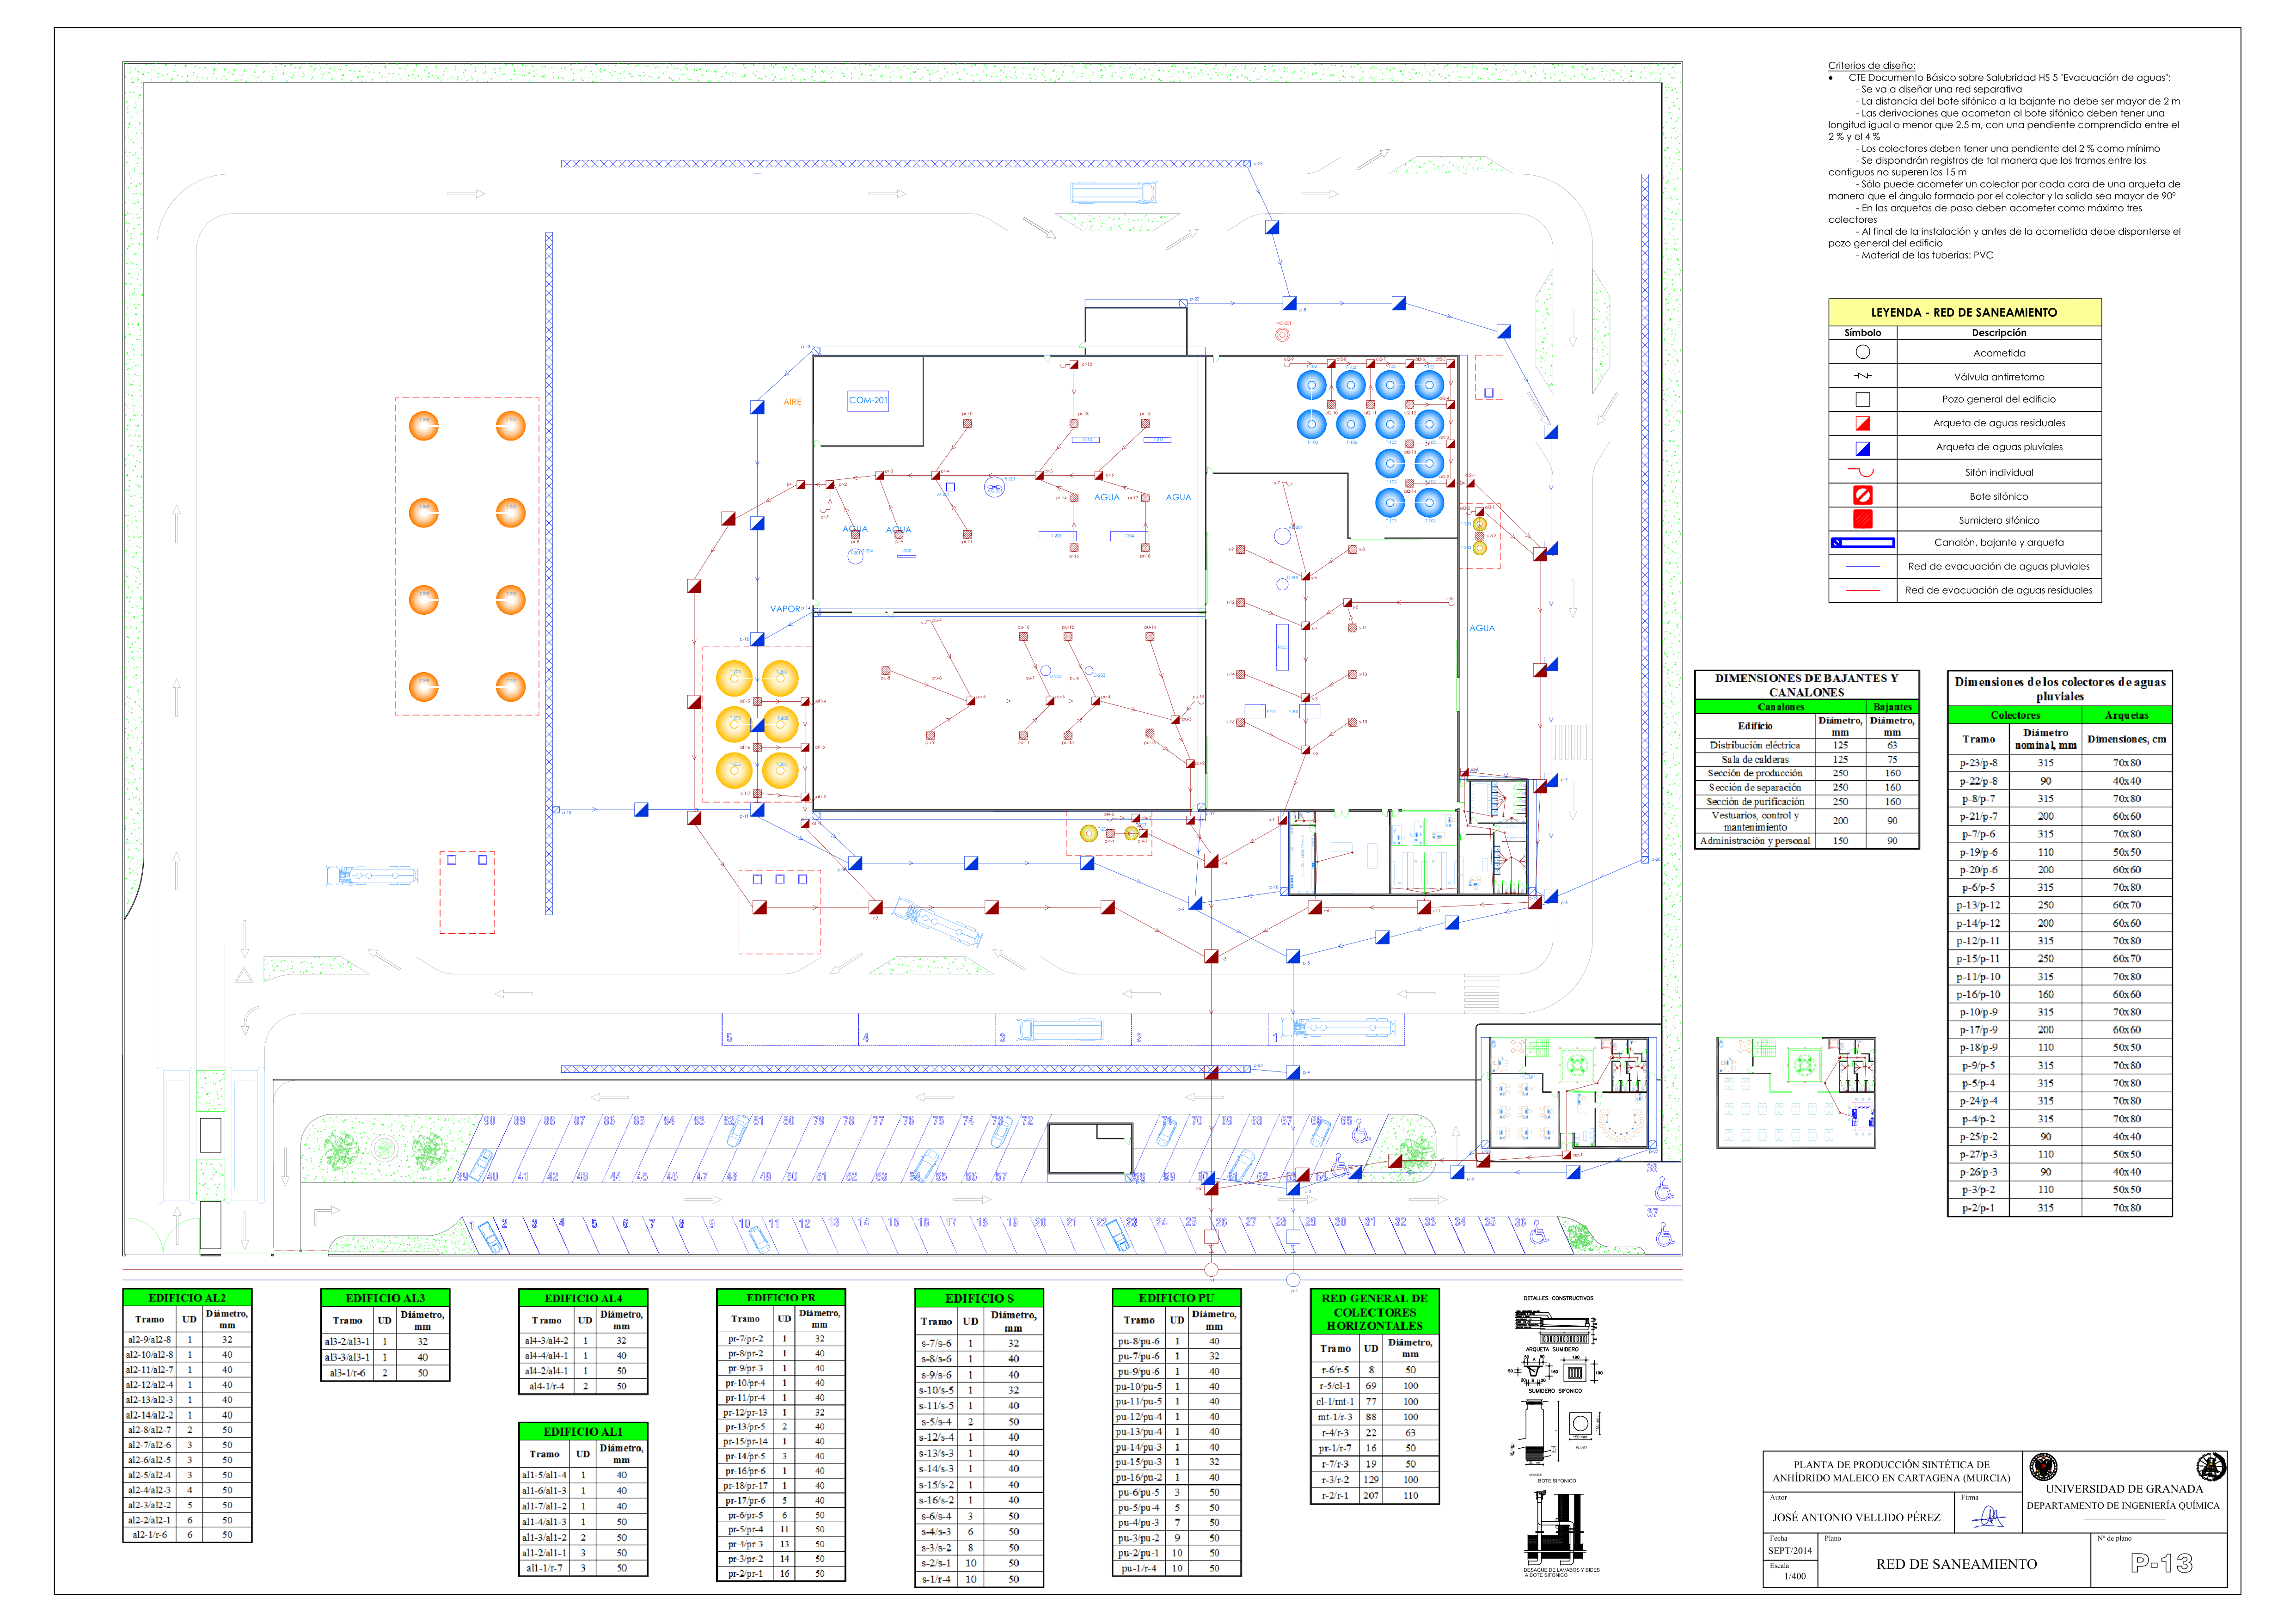
\includegraphics[width=0.95\linewidth,height=0.85\textheight,keepaspectratio]{Doc/Planos/plano_saneamiento_planta_land.png}
\caption{Plano de Planta General de la Red de Saneamiento Industrial: Colectores separativos de fecales, pluviales y vertidos de proceso, arquetas de paso, pozos de registro y acometida municipal (\cite{vellido_perez_2014}).}
\label{fig:plano_general_saneamiento}
\end{figure}
\end{landscape}


\section{Normativa Medioambiental e Hidráulica de Vertidos}

\subsection{Texto Refundido de la Ley de Aguas (TRLA) y Canon de Control de Vertidos}
El TRLA consagra en sus artículos 100 a 108 el principio de que todo vertido al dominio público hidráulico requiere previa autorización administrativa otorgada por el organismo de cuenca correspondiente (Confederación Hidrográfica):
\begin{itemize}
    \item \textbf{Canon de Control de Vertidos (art.~113 TRLA y arts.~289--295 RDPH):} Todo vertido al dominio público hidráulico devenga anualmente este canon, destinado al estudio, control, protección y mejora del medio receptor. Su importe es el producto del volumen de vertido autorizado por el precio unitario de control de vertido, descontando el volumen de agua efectivamente reutilizado en el período impositivo (art.~291 RDPH):
    \begin{equation}
        C_{\text{CV}} = (V_{\text{autorizado}} - V_{\text{reutilizado}}) \cdot P_{\text{u}}, \qquad P_{\text{u}} = P_{\text{b}} \cdot K
        \label{eq:canon_vertido}
    \end{equation}
    donde:
    \begin{itemize}
        \item $V_{\text{autorizado}}$ es el volumen anual de vertido fijado en la autorización ($\text{m}^3/\text{año}$) y $V_{\text{reutilizado}}$ el volumen efectivamente reutilizado.
        \item $P_{\text{b}}$ es el precio básico por metro cúbico del art.~113.3 TRLA, actualizable mediante las Leyes de Presupuestos Generales del Estado. Los valores vigentes aplicados por los organismos de cuenca son $0{,}01751$\,€/m$^3$ para agua residual urbana y $0{,}04377$\,€/m$^3$ para \textbf{agua residual industrial}.
        \item $K$ es el coeficiente de mayoración o minoración del \textbf{anexo IV del RDPH}, obtenido como producto de tres factores: la \textit{naturaleza y características} del vertido (urbano o industrial; en el caso industrial, según la clase de actividad y la presencia de sustancias peligrosas), el \textit{grado de contaminación} (según exista o no un tratamiento adecuado) y la \textit{calidad ambiental del medio receptor} (categoría de la zona de vertido). Tras el Real Decreto-ley 4/2023, el coeficiente de mayoración no puede ser superior a 5 (art.~291.3 RDPH), y los nuevos factores del anexo IV fijados por el RD 665/2023 se aplican a los cánones devengados desde el 31 de diciembre de 2025 (disposición transitoria duodécima).
    \end{itemize}

    \item \textbf{Valoración de Daños al Dominio Público Hidráulico (Infracciones y Vertidos No Autorizados):} Debe distinguirse el canon tributario ordinario de la fórmula oficial de \textbf{valoración e indemnización por daños al medio hídrico} tipificada en los artículos 325 y siguientes y detallada en el \textbf{Anexo V del RDPH} (modificado por el RD 665/2023), aplicable ante accidentes, derrames o vertidos no autorizados:
    \begin{equation}
        V_{\text{Daño}} \text{ (€)} = \text{CTEC} \cdot V \cdot K_{\text{pv}} \cdot K_{\text{m}} = 0{,}12\text{ €}/\si{m^3} \cdot (Q \cdot t) \cdot K_{\text{pv}} \cdot K_{\text{m}}
        \label{eq:valoracion_danos}
    \end{equation}
    donde:
    \begin{itemize}
        \item $\text{CTEC} = 0{,}12\text{ €}/\si{m^3}$ es el coste teórico unitario del tratamiento de vertido para evitar la contaminación.
        \item $V = Q \cdot t$ es el volumen vertido en $\si{m^3}$ ($Q$ caudal en $\text{m}^3/\text{día}$ y $t$ duración en días).
        \item $K_{\text{pv}}$ es el coeficiente adimensional de peligrosidad del vertido establecido en el \textbf{Anexo V.A} según la tipología de las sustancias vertidas (DQO, toxicidad, metales pesados, etc.).
        \item $K_{\text{m}}$ es el coeficiente adimensional relativo a la clasificación y sensibilidad ambiental del medio receptor incluido en el \textbf{Anexo V.B} (zonas de protección, estado de las masas de agua y acuíferos).
    \end{itemize}
\end{itemize}


\subsection{Reglamento del Dominio Público Hidráulico (RD 849/1986 y RD 665/2023)}
La reforma del RDPH consolidada por el \textbf{Real Decreto 665/2023} ha elevado sensiblemente las exigencias técnicas aplicables a las plantas químicas e industriales:
\begin{itemize}
    \item \textbf{Límites de vertido:} Los valores límite de emisión no son una tabla general del RDPH: se fijan caso por caso en la autorización de vertido del organismo de cuenca, atendiendo a las mejores técnicas disponibles (\cite{CWW_BREF_2016}) y a los objetivos de calidad del medio receptor (\cite{TRLA2001, RDPH1986}).
    \item \textbf{Protección de aguas subterráneas frente a contaminación puntual:} La reforma incorpora valores de referencia para aguas subterráneas y, si se superan, exige un Análisis Cuantitativo de Riesgos (ACR) que determine las medidas correctoras. Para una planta química esto obliga a justificar la contención de derrames y a prever controles piezométricos; el articulado concreto debe consultarse en el texto consolidado del RDPH (\cite{RDPH1986}).
    \item \textbf{Perímetros de protección:} El RDPH regula la delimitación de perímetros de protección de captaciones de agua subterránea destinadas a consumo humano. Si la planta se abastece de un pozo propio para uso industrial, esta obligación no se aplica automáticamente, pero la concesión y la ubicación del pozo deben evaluarse frente a los perímetros existentes en la zona (\cite{RDPH1986}).
\end{itemize}

\subsection{Directiva (UE) 2024/3019: Tratamiento Cuaternario y Responsabilidad Ampliada (RAP)}
La Directiva (UE) 2024/3019, que refunde el marco europeo de tratamiento de aguas residuales urbanas, introduce dos novedades con efecto indirecto sobre la industria química (por sus vertidos a redes urbanas) (\cite{DirectivaUE_2024_3019}):
\begin{itemize}
    \item \textbf{Tratamiento cuaternario:} Las depuradoras urbanas de mayor tamaño (y otras en zonas sensibles) deben eliminar microcontaminantes (fármacos, tensioactivos, disruptores endocrinos, etc.) mediante procesos como oxidación avanzada o adsorción en carbón activo.
    \item \textbf{Responsabilidad ampliada del productor:} Los productores de sectores identificados como principales fuentes de microcontaminantes (en particular farmacéutico y cosmético) deben sufragar como mínimo el $80\text{ \%}$ del coste adicional del tratamiento cuaternario.
\end{itemize}

\subsection{Huella Hídrica y Ecoeficiencia según Norma UNE-EN ISO 14046}
La norma internacional \textbf{UNE-EN ISO 14046} define los principios de evaluación del ciclo de vida (ACV) aplicados al uso del agua en plantas industriales. En la ingeniería de detalle del proyecto se cuantifican:
\begin{equation}
    \text{HH}_{\text{total}} = \text{HH}_{\text{azul}} + \text{HH}_{\text{verde}} + \text{HH}_{\text{gris}}
\end{equation}
donde la \textbf{Huella Azul} mide el volumen consumido de recursos hídricos de la red o acuífero evaporado o incorporado al producto; la \textbf{Huella Verde} corresponde al agua de lluvia almacenada; y la \textbf{Huella Gris} representa el volumen teórico de agua limpia necesario para asimilar la carga contaminante de los efluentes vertidos hasta alcanzar los estándares de calidad del cauce receptor.

\subsection{Conclusiones Normativas para el Proyecto de Ingeniería}
El cumplimiento integrado de esta arquitectura jurídica y técnica impone en la memoria, pliego y planos del proyecto:
\begin{enumerate}
    \item La justificación técnica formal de la no toxicidad de los materiales en contacto con agua potable (RD 3/2023).
    \item El dimensionamiento higiénico de las torres y balsas de refrigeración según el PPCL exigido por el RD 487/2022.
    \item La segregación y modelado hidráulico estricto de las 4 redes de saneamiento (fecales, pluviales limpias, pluviales contaminadas y vertidos de proceso), reflejando con exactitud la simbología normalizada de arquetas, separadores y pozos (CTE DB-HS 5, UNE-EN 752, UNE-EN ISO 129-1:2019).
    \item La instalación perimetral de un pozo oficial homologado de control y aforo continuo de vertidos para la supervisión ambiental por la administración hidráulica (TRLA / RDPH).
\end{enumerate}


%
% ==========================================================================
% CAPITULO 6 COMENTADO TEMPORALMENTE (PRESERVADO PARA CONSULTA)
% ==========================================================================

\chapter{Conclusiones e Integración Técnica en el Proyecto}
\label{cap:conclusiones_integracion}

\section{Síntesis de Decisiones de Ingeniería}

El estudio técnico desarrollado para la gestión de servicios básicos de abastecimiento y saneamiento en el complejo industrial permite consolidar las siguientes directrices y decisiones de ingeniería:

\begin{enumerate}
    \item \textbf{Estrategia de Suministro Mixta y Blindaje Hídrico:}
          \begin{itemize}
              \item \textbf{Red Municipal para Agua Sanitaria y de Consumo:} Garantiza la máxima seguridad bromatológica, microbiológica y toxicológica en estricto cumplimiento del Real Decreto 3/2023 para el personal y formulaciones sensibles, sin exigir la implantación ni el coste operativo de complejas estaciones potabilizadoras en la parcela.
              \item \textbf{Captación Propia Concesionada para Procesos Gruesos y Refrigeración:} Siempre que exista disponibilidad hidrogeológica validada por la Confederación Hidrográfica, la explotación de un pozo de sondeo profundo para el circuito de refrigeración y limpiezas primarias minimiza de forma decisiva los costes de explotación ($OPEX$).
          \end{itemize}

    \item \textbf{Robustez del Diseño Hidráulico Interior:}
          \begin{itemize}
              \item La previsión de un \textbf{depósito partido en dos compartimentos simétricos independientes con colector exterior en bypass} garantiza la continuidad operativa ininterrumpida de la factoría durante las tareas de mantenimiento, vaciado y desinfección preventiva contra \textit{Legionella} (RD 487/2022).
              \item La intercalación obligatoria de una \textbf{desconexión hidráulica atmosférica de rotura de carga (Air Gap Break Tank, UNE-EN 1717)} en la alimentación del depósito elimina de manera absoluta cualquier riesgo de contaminación por reflujo o contrasifonado hacia la red pública.
              \item La estación de sobreelevación multi-bomba en paralelo ($2+1$) con variadores electrónicos de frecuencia (VFD) asegura una consigna de presión constante de $3.5\text{ a }4.0\text{ bar}$ en los colectores de planta, modulando la potencia eléctrica al consumo instantáneo real y con una bomba de reserva activa al $100\%$.
          \end{itemize}

    \item \textbf{Conformidad Sanitaria y Medioambiental Exhaustiva:}
          \begin{itemize}
              \item La especificación de materiales homologados en listas positivas (PE 100 PN 16 exterior, PP-R y multicapa en locales húmedos, acero inoxidable AISI 316L en proceso) elimina cualquier fenómeno de migración química, corrosión o incrustación.
              \item La red de saneamiento separativa y la estación depuradora de aguas residuales industriales (EDARI) garantizan que los efluentes vertidos a la red municipal cumplan rigurosamente los parámetros límite de vertido (DBO$_5$, DQO, sólidos en suspensión y metales pesados), salvaguardando la responsabilidad civil y ambiental del promotor.
          \end{itemize}
\end{enumerate}

\chapter*{Declaración sobre el Uso de Inteligencia Artificial Generativa}
\addcontentsline{toc}{chapter}{Declaración sobre el Uso de Inteligencia Artificial Generativa}

En cumplimiento de las buenas prácticas académicas y las directrices institucionales adaptadas a la norma APA (7.ª edición) para la citación de herramientas de Inteligencia Artificial Generativa (IAG), se declara formalmente la asistencia tecnológica empleada en la elaboración del presente documento.

\section*{Herramientas y Modelos Empleados}
Para la preparación, estructuración y verificación de este trabajo se ha contado con la asistencia de los siguientes modelos de lenguaje de gran escala (LLM):
\begin{itemize}
    \item \textbf{Google Gemini 3.8 Flash (Low) y Google Gemini Argon (Low)} (\cite{google_gemini_2026}): Empleados como sistemas principales para la búsqueda preliminar de normativa técnica estatal y autonómica, redacción inicial de apartados, estructuración conceptual y apoyo en el modelado de diagramas en TikZ.
    \item \textbf{Anthropic Claude Opus 5.5 (Mid)} (\cite{anthropic_claude_2026}): Utilizado de forma complementaria y en menor medida para la contrastación de fuentes jurídicas complejas, validación cruzada de criterios de diseño del Código Técnico de la Edificación y refinamiento crítico de fórmulas de vertidos.
\end{itemize}

\section*{Naturaleza y Alcance de la Asistencia}
El autor declara que la Inteligencia Artificial Generativa ha sido utilizada exclusivamente como herramienta auxiliar de asistencia en la búsqueda bibliográfica, la revisión de estilo y composición documental y comprobación cruzada de requisitos legales. Todo el contenido teórico, fórmulas matemáticas, decisiones de diseño, redacción final y conclusiones han sido íntegramente revisados, contrastados con las fuentes oficiales primarias (BOE, Confederaciones Hidrográficas, Guías Técnicas y Normas UNE) y asumidos bajo la exclusiva responsabilidad del autor.

\vspace{1.5em}
\noindent\textbf{Declaración Final del Estudiante:}
\begin{itemize}
    \item[$\square$] Declaro explícitamente que no se ha utilizado Inteligencia Artificial Generativa en la elaboración de este trabajo.
    \item[$\boxtimes$] \textbf{Declaro explícitamente que el contenido registrado en la presente declaración es fidedigno y abarca la totalidad del uso de IAG realizado para este trabajo.}
\end{itemize}

\vspace{2.5em}
\noindent\begin{tabularx}{\textwidth}{l X l}
\textbf{Firma del Estudiante:} & & \textbf{Fecha:} 31/10/2026 \\
\cline{1-3}
Christian Pérez Hita & & \\
\end{tabularx}

\newpage

\printbibliography[heading=bibintoc, title={Referencias Bibliográficas y Legislativas}]

\end{document}
